% \documentclass[acmsmall,screen,review,anonymous]{acmart}
\documentclass[format=sigconf, screen=true, review=false]{acmart}
% \citestyle{acmauthoryear} 

% \setcopyright{rightsretained} 
% \acmJournal{PACMMOD}
% \acmYear{2023} \acmVolume{1} \acmNumber{2} \acmArticle{150} \acmMonth{6} \acmPrice{}\acmDOI{10.1145/3589295}

%% \BibTeX command to typeset BibTeX logo in the docs \AtBeginDocument{%
\AtBeginDocument{%
\providecommand\BibTeX{{%
Bib\TeX}}}

\makeatletter
\gdef\@copyrightpermission{
  \begin{minipage}{0.2\columnwidth}
   \href{https://creativecommons.org/licenses/by/4.0/}{
\includegraphics[width=0.90\textwidth]{fig/4ACM-CC-by-88x31.eps}}
  \end{minipage}\hfill
  \begin{minipage}{0.8\columnwidth}
   \href{https://creativecommons.org/licenses/by/4.0/}{This work is licensed under a Creative Commons Attribution International 4.0 License.}
  \end{minipage}
  \vspace{5pt}
}
\makeatother

% For June V1mod112-V1mod188 (cycle C), use
\received{October 2022}
\received[revised]{January 2023}
\received[accepted]{February 2023}	

\author{Yisu Remy Wang}
\affiliation{
  \institution{University of California, Los Angeles}
  \country{USA}
}
% \email{remywang@cs.ucla.edu}
\authornote{Work done while at University of Washington.}

\author{Max Willsey}
\affiliation{
  \institution{University of California, Berkeley}
  \country{USA}
}
% \email{mwillsey@eecs.berkeley.edu}
\authornotemark[1]


\author{Dan Suciu}
\affiliation{
  \institution{University of Washington}
  \country{USA}
}
% \email{suciu@cs.washington.edu}

\keywords{Worst-case optimal join}

\newcommand{\calH}{\mathcal H}
\newcommand{\calD}{\mathcal D}
\newcommand{\calP}{\mathcal P}
\newcommand{\calV}{\mathcal V}
\newcommand{\calX}{\mathcal X}
\newcommand{\calY}{\mathcal Y}
\newcommand{\calE}{\mathcal E}
\newcommand{\calF}{\mathcal F}
\newcommand{\calT}{\mathcal T}

\newcommand{\mv}[1]{\mathbf{#1}}

\usepackage{tikz}
\usepackage[inline]{enumitem}
% \usepackage{amssymb}
\usepackage[font=small,labelfont=bf]{caption}
\usepackage{subcaption}
\usepackage{algorithm}
\usepackage[noend]{algpseudocode}
% \usepackage{stmaryrd}

\usepackage{bm} % bold math fonts, e.g. $\bm \Sigma$ will give a bold-face $\Sigma$

\usepackage{graphics}
\graphicspath{{_build/}{fig/}}

% \usepackage{syntax}

\setlength {\marginparwidth }{2cm}
\usepackage[colorinlistoftodos]{todonotes}

% \usepackage{hyperref}
% \def\algorithmautorefname{Algorithm}
% \def\sectionautorefname{Section}
% \def\subsectionautorefname{Section}
% \def\subsubsectionautorefname{Section}

\usepackage{listings} % requires pygment syntax highlighting

\lstset{
  columns=flexible,
  keepspaces=true,
  numbers=left,
  numberstyle=\ttfamily\scriptsize\color{black!40},
  showstringspaces=false,
  stringstyle=\slshape\color{green!40!black},
  basicstyle=\ttfamily\small,
  language=Python,
  deletekeywords=[2]{map, iter, vars, tuple},
  morekeywords={self, interface},
  commentstyle=\slshape\color{black!60},
  mathescape=true,
  tabsize=2,
}

% \lstset{
%   language=Python,
%   columns=flexible,
%   keepspaces=true,
%   showstringspaces=false,
%   stringstyle=\slshape\color{green!40!black},
%   morekeywords={*, self},
%   commentstyle=\slshape\color{black!60},
%   tabsize=2,
%   xleftmargin=6.5mm,
% }

\usepackage{xspace}

\newcommand{\FJ}{\textsf{Free Join}\xspace}
\newcommand{\GJ}{\textsf{Generic Join}\xspace}
\newcommand{\WCOJ}{\textsf{WCOJ}\xspace}
\newcommand{\GHT}{\textsf{GHT}\xspace}
\newcommand{\GHTs}{\textsf{GHT}s\xspace}
\newcommand{\COLT}{\textsf{COLT}\xspace}
\newcommand{\COLTs}{\textsf{COLT}s\xspace}
\newcommand{\cd}{\text{ :- }}
\newcommand{\setof}[2]{\{{#1}\mid{#2}\}}        % Set (as in \setof{x}{x>0}).
\newcommand{\set}[1]{\{#1\}}        % Set (as in \setof{x}{x>0}).
\newcommand{\loopi}{\circlearrowleft}
\newcommand{\hjacyc}{8x\xspace}
\newcommand{\hjcyc}{?x\xspace}
\newcommand{\gjacyc}{?x\xspace}
\newcommand{\gjcyc}{?x\xspace}
\newcommand{\gjbad}{?x\xspace}
\newcommand{\hjbad}{?x\xspace}
\newcommand{\imdbavgfjbj}{2.94x\xspace}
\newcommand{\imdbavgfjgj}{9.61x\xspace}
\newcommand{\imdbmaxfjbj}{19.36x\xspace}
\newcommand{\imdbmaxfjgj}{31.6x\xspace}
\newcommand{\imdbminfjbj}{0.85x\xspace}
\newcommand{\imdbmaxbjfj}{17\%\xspace}
\newcommand{\imdbminfjgj}{2.63x\xspace}


% \def\drawplusplus#1#2#3{\hbox to 0pt{\hbox to #1{\hfill\vrule height #3 depth
%       0pt width #2\hfill\vrule height #3 depth 0pt width #2\hfill
%       }}\vbox to #3{\vfill\hrule height #2 depth 0pt width
%       #1 \vfill}}
%       %Poor man's typography
% \def\concat{\mathrel{\drawplusplus {12pt}{0.4pt}{5pt}}}
%       %It would be better to specify these in font-relative measures, but it 
%       %probably doesn't scale anyway.

% \newcommand{\sys}{\texttt{Qry}\xspace}
% \newcommand{\clover}{\tikz{\draw (0, 0) -- (90:0.7ex); \draw (0,0) -- (210:0.7ex);\draw(0,0) -- (330:0.7ex)}}

%%% Local Variables:
%%% mode: latex
%%% TeX-master: "main"
%%% End:


% \usepackage[capitalize,nameinlink]{cleveref}
% \def\drawplusplus#1#2#3{\hbox to 0pt{\hbox to #1{\hfill\vrule height #3 depth
%       0pt width #2\hfill\vrule height #3 depth 0pt width #2\hfill
%       }}\vbox to #3{\vfill\hrule height #2 depth 0pt width
%       #1 \vfill}}
%       %Poor man's typography
% \def\concat{\mathrel{\drawplusplus {12pt}{0.4pt}{5pt}}}
%       %It would be better to specify these in font-relative measures, but it
%       %probably doesn't scale anyway.

\newcommand{\rw}[1]{\todo[inline,color=yellow]{\textsf{#1} \hfill \textsc{--Remy}}}
\newcommand{\ds}[1]{\todo[inline,color=orange]{\textsf{#1} \hfill \textsc{--Dan}}}
% \newcommand{\ds}[1]{\todo[color=orange]{\textsf{#1} \hfill \textsc{--Dan}}}
% \newtheorem{theorem}{Theorem}
\newcommand{\yell}[1]{{\color{red} \textbf{#1}}}
\newcommand{\dan}[1]{{\color{red} \textbf{#1}}}
\newcommand{\remy}[1]{{\color{orange} \textbf{#1}}}

\begin{document}

% \title{Comparing and Unifying Worst-Case Optimal Join with Traditional Join Algorithms, Part I: Hash Joins}
\title{\FJ: Unifying Worst-Case Optimal and Traditional Joins}

\begin{abstract}
  Over the last decade, worst-case optimal join (\WCOJ) algorithms have
emerged as a new paradigm for one of the most fundamental challenges
in query processing: computing joins efficiently.  Such an algorithm
can be asymptotically faster than traditional binary joins, all the
while remaining simple to understand and implement.  However, they
have been found to be less efficient than the old paradigm,
traditional binary join plans, on the typical acyclic queries found in
practice.
In an effort to unify and generalize the two paradigms,
we proposed a new framework, called \FJ, in our SIGMOD 2023 paper.
Not only does \FJ unite the worlds of traditional and worst-case optimal
join algorithms, it uncovers optimizations and evaluation strategies
that outperform both.

In this article, we approach \FJ from the traditional perspective
of binary joins, and re-derive the more general framework
via a series of gradual transformations.
We hope this perspective from the past can help practitioners
better understand the \FJ framework,
and find ways to incorporate some ideas into their own systems.

% Some database systems that support \WCOJ use a hybrid
% approach: use \WCOJ to process the cyclic subparts of the query (if
% any), and rely on traditional binary joins otherwise.  In this paper
% we propose a new framework, called \FJ, that unifies the two
% paradigms.  We describe a new type of plan, a new data structure
% (which unifies the hash tables and tries used by the two paradigms),
% and a suite of optimization techniques.  Our system, implemented in
% Rust, matches or outperforms both traditional binary joins and \WCOJ on
% standard query benchmarks.
\end{abstract}

\begin{CCSXML}
  <ccs2012>
  <concept>
  <concept_id>10002951.10002952.10003190.10003192.10003426</concept_id>
  <concept_desc>Information systems~Join algorithms</concept_desc>
  <concept_significance>500</concept_significance>
  </concept>
  </ccs2012>
\end{CCSXML}

\ccsdesc[500]{Information systems~Join algorithms}

\maketitle

\section{Introduction}\label{sec:intro}

% \ds{break this long paragraph into smaller ones}
Over the last decade, worst-case optimal join (\WCOJ)
algorithms~\cite{DBLP:conf/pods/NgoPRR12, DBLP:conf/icdt/Veldhuizen14,
  DBLP:journals/sigmod/NgoRR13, DBLP:conf/pods/000118} have emerged as
a breakthrough in one of the most fundamental challenges in query
processing: computing joins efficiently.  Such an algorithm can be
asymptotically faster than traditional binary joins, all the while
remaining simple to understand and
implement~\cite{DBLP:journals/sigmod/NgoRR13}.  These algorithms
opened up a flourishing field of research, leading to both theoretical
results~\cite{DBLP:journals/sigmod/NgoRR13,DBLP:conf/pods/Khamis0S17}
and practical
implementations~\cite{DBLP:conf/icdt/Veldhuizen14,DBLP:journals/tods/AbergerLTNOR17,DBLP:journals/pvldb/FreitagBSKN20, DBLP:journals/pvldb/MhedhbiS19}.

Over time, a common belief took hold:
``\WCOJ is designed for cyclic queries''.
This belief is rooted in the observation that
\WCOJ enjoys lower asymptotic complexity
than traditional algorithms for cyclic queries~\cite{DBLP:journals/sigmod/NgoRR13},
but when the query is acyclic,
classic algorithms like the Yannakakis algorithm~\cite{DBLP:conf/vldb/Yannakakis81}
are already asymptotically optimal.
Moreover, traditional binary join algorithms have benefited from
decades of research and engineering.
Techniques like column-oriented layout, vectorization,
and query optimization
have contributed compounding constant-factor speedups,
making it challenging for \WCOJ to be competitive in practice.
% \ds{Can you be specific and explain this was done in Hyper}
% This has lead many instantiations of \WCOJ,
% including Umbra~\cite{DBLP:journals/pvldb/FreitagBSKN20},
% Emptyheaded~\cite{DBLP:journals/tods/AbergerLTNOR17}, and Graphflow~\cite{DBLP:journals/pvldb/MhedhbiS19},
% to adopt a hybrid approach:
% using \WCOJ to process parts of the query,
% % \rw{Umbra actually does not use \WCOJ only for cycles.
% % It relies on the optimizer to detect skew, and use \WCOJ 
% %   for skewed joins.}
% and resorting to traditional algorithms (usually binary join)
% for the rest.
% Having two different algorithms in the same system
% requires changing and potentially duplicating existing infrastructure
% like the query optimizer.
% This introduces complexity, and hinders the adoption of \WCOJ.

The dichotomy of \WCOJ versus binary join has led researchers
and practitioners to view the algorithms as opposites.
In our SIGMOD 2023 paper~\cite{10.1145/3589295},
we broke down this dichotomy with a new framework called \FJ
that unifies \WCOJ and binary join.
We proposed new data structures, evaluation algorithms,
and optimizations to make \FJ outperform both binary join and \WCOJ.
% we design an algorithm to convert any binary join plan to a \FJ plan
% that runs as fast or faster; we design a new data structure called
% \COLT (for \emph{Column-Oriented Lazy Trie}), adapting the classic
% column-oriented layout to improve the trie data structure used in
% \WCOJ; and we propose a vectorized execution algorithm for \FJ.

In this article, we review \FJ from a different perspective:
starting from the traditional binary join algorithm,
we apply a series of gradual transformations
to arrive at the \FJ algorithm as well as the \WCOJ algorithm.
We hope this perspective from the past can help practitioners
better understand \FJ,
and pave the way for its adoption in existing systems.


% \begin{figure}
%   \centering
%   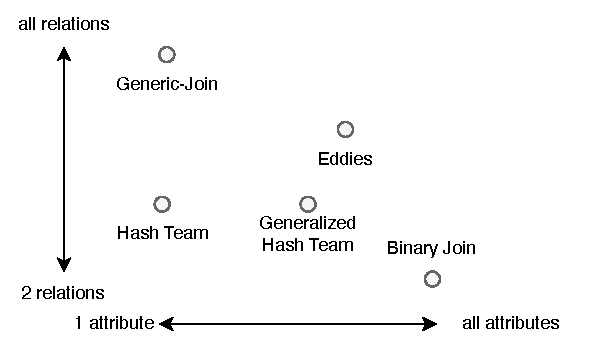
\includegraphics[width=0.55\linewidth]{free-join.pdf}
%   \caption{Design space of join algorithms.}
%   \label{fig:design-space}
% \end{figure}

% To explain our contributions we provide some context.
% %
% In this work, we focus on algorithms based on hashing,
% and choose \GJ~\cite{DBLP:journals/sigmod/NgoRR13} as a representative of \WCOJ algorithms.
% A crucial difference between \GJ and binary join lies
% in the way they process each join operation.
% Binary join processes two relations at a time,
% and joins on \emph{all attributes}
% in the join condition between these two relations.
% In contrast, \GJ processes one attribute at a time,
% and joins \emph{all relations} that share that attribute.
% This suggests a design space of join algorithms,
% where each join operation may process any
% number of attributes and relations.
% Figure~\ref{fig:design-space} shows this design space
% which also covers classic multiway join algorithms
% like Hash Team~\cite{DBLP:conf/vldb/GraefeBC98},
% Generalized Hash Team~\cite{DBLP:conf/vldb/KemperKW99}
% and Eddies~\cite{DBLP:conf/sigmod/HellersteinA00}.
% Being able to join on any number of variables and relations
% frees us from the constraints of all existing algorithms
% mentioned above.
% % } \yell{I suggest removing the boldface}

% Our new framework, \FJ,
% covers the entire design space,
% thereby generalizing and unifying existing algorithms.
% The starting observation is that the execution of a left-deep linear
% binary join plan is already very similar to \GJ.
% While \GJ (reviewed in Sec.~\ref{sec:background}) is traditionally specified as a series of nested loops~\cite{DBLP:journals/sigmod/NgoRR13},
% the push-based model~\cite{DBLP:journals/pvldb/Neumann11,DBLP:journals/pvldb/KerstenLKNPB18} for executing a left-deep linear binary plan
% is also implemented, similarly, as nested loops.
% % \rw{Should I add an example of the loop nest, or is that too much detail?}
% % \ds{Not here, but please explain this point again in the technical
% %   sections, and give an example there.}
% The two algorithms also process each join operation similarly:
% each binary hash join iterates over tuples on one relation,
% and for each tuple probes into the hash table of another relation;
% each loop level in \GJ iterates over the keys of a certain trie,
% and probes into several other tries for each key.
% This inspired us to unify hash tables and hash tries into the same data structure,
% and develop \FJ using iteration and probing as key operations.
% This finer-grained view of join algorithms allows \FJ
% to generalize and unify existing algorithms,
% while precisely capturing each of them.

% \FJ takes as input an already optimized binary join plan, and
% converts it into a new kind of plan that we call a \FJ plan.  It
% then optimizes the \FJ plan, resulting in a plan that sits in
% between binary join and \GJ, combining the benefits of both.  On one
% hand \FJ takes full advantage of the design space in
% Figure~\ref{fig:design-space}.  On the other hand, by starting from
% an already optimized binary plan, \FJ takes advantage of existing
% cost-based optimizers; in our system we used binary plans produced by
% the optimizer of DuckDB~\cite{DBLP:conf/cidr/RaasveldtM20,DBLP:conf/vldb/Raasveldt22}.

% Next, we address the main source of
% inefficiency in \GJ: the need to construct a trie on each relation
% in the query.  In contrast,
% a binary join plan needs to build a hash map only for each relation
% on the right-hand side of a join,
% and simply iterates over the relation on the left.
% In practice, trie-building has been observed to be a major
% bottleneck for \GJ~\cite{DBLP:journals/pvldb/MhedhbiS19,DBLP:journals/pvldb/FreitagBSKN20},
% making it slower than binary join.
% This is because each trie is more expensive to build than a hash map,
% and the left relation is usually chosen to be a large relation
% by the query optimizer.
% One simple optimization in \FJ is that we do not built a trie for
% tables that are left children, mimicking the binary plans.
% %
% However, we go a step further, and introduce the {\em Column-Oriented
%     Lazy Trie} (\COLT) data structure, which builds the inner subtries
% lazily, by creating each subtrie on demand.
% We note that this builds on an earlier idea
% in~\cite{DBLP:journals/pvldb/FreitagBSKN20}.  As the name suggests,
% \COLT adapts the lazy trie data structure
% in~\cite{DBLP:journals/pvldb/FreitagBSKN20} to use a column-oriented
% layout.  And unlike the original lazy trie which builds at least one
% trie level per table, \COLT completely eliminates the cost of trie
% building for left tables.


% Finally, we describe a method for incorporating vectorized
% processing in \FJ, allowing it to collect multiple data values
% before entering the next iteration level.
% The standard \GJ processes one data value at a time, but, as is the
% case in traditional query engines, this leads to poor cache
% locality.
% Vectorized execution~\cite{DBLP:conf/icde/PadmanabhanAMJ01} was proposed for binary join
% to improve its locality by processing data values in batch.
% By breaking down join operations into iterations and probes,
% \FJ gives rise to a simple vectorized execution algorithm
% that breaks each iteration into chunks and groups together
% batches of probes.
% Our proposal is to our knowledge the first vectorized execution algorithm for \GJ.

% We implemented \FJ as a standalone Rust library, and
% compared it with two baselines:
% \begin{enumerate*}
%   \item our own \GJ implementation in Rust, and
%   \item the binary hash join implemented in
%         DuckDB~\cite{DBLP:conf/cidr/RaasveldtM20,DBLP:conf/vldb/Raasveldt22},
%         a state-of-the-art in-memory database.
% \end{enumerate*}
% %%%%%%%%%% No need for experimental details here, just some highlights
% %%%   We conduct experiments on the popular Join Order
% %%%   Benchmark~\cite{DBLP:journals/pvldb/LeisGMBK015} and the
% %%%   LSQB~\cite{} benchmark.
% We found that, on acyclic queries, \FJ is up to \imdbmaxfjbj
% faster than binary join, and up to \imdbmaxfjgj faster than \GJ; on
% cyclic queries, \FJ is up to 15.45x faster than binary join, and up
% to 4.08x faster than \GJ.
% % \FJ also retains its advantage even when the optimizer chooses a poor plan.
% %%%   We conduct additional experiments on
% %%%   synthetic data for star and chain queries, as well as ablation
% %%%   studies on the optimizations.  Finally, we compare \FJ and binary
% %%%   hash join on their robustness against bad query plans.  Given a bad
% %%%   query plan, \FJ runs up to \hjbad and \gjbad faster than binary join
% %%%   and \GJ, respectively.

% While optimizers for binary plans have been developed and improved
% over decades~\cite{DBLP:conf/sigmod/SelingerACLP79}, little
% is known about optimizing \GJ.  A \GJ plan consists of a total order
% on its variables, and its run time does depend on the choice of this
% order.  But since the theoretical analysis of \GJ guarantees worst
% case optimality for {\em any} variable order, it is a folklore
% belief that \GJ is more robust than binary join plans to poor
% choices of the optimizer.  We also conduced experiments measuring
% the robustness of the three types of plans (binary, \GJ, \FJ) to
% poor choices of the optimizer.  We found that \GJ is indeed the
% least sensitive, while \FJ, like binary joins, suffers more from the
% poor optimization choices of the optimizer, since both rely on a
% cost-based optimized plan.  However, \GJ starts from worse baseline
% than \FJ.  In other words, \FJ takes better advantage of a good
% plan, when available, than \GJ does.



% In summary, we make the following contributions in this paper:
% % \ds{Please reference the sections where these contributions are
% %   described.  Currently the do NOT align with the contributions
% %   mentioned earlier and discussed in the introduction.  This needs to
% %   be fixed.}
% % \rw{Fixed.}
% \begin{enumerate}
%   \item \FJ, a framework unifying existing join algorithms (Section~\ref{sec:free-join}).
%   \item An algorithm to converting any binary join plan into an
%         optimized \FJ plan (Section~\ref{sec:bj-to-fj}).
%   \item \COLT, a column-oriented lazy trie data structure (Section~\ref{sec:colt}).
%   \item A vectorized execution algorithm for \FJ (Section~\ref{sec:vectorized-execution}).
%   \item Experiments evaluating the algorithms and optimizations (Section~\ref{sec:eval}).
% \end{enumerate}
\section{From Binary Join to Free Join}\label{sec:background}

\begin{figure}
  \begin{align*}
    Q_{\clubsuit}(x,a,b,c) \cd R(x,a),S(x,b),T(x,c).
  \end{align*}
  \begin{center}
    \begin{tabular}{c}
      \begin{lstlisting}[language=SQL, numbers=none]
SELECT * FROM R, S, T WHERE R.x = S.x AND S.x = T.x
\end{lstlisting}
    \end{tabular}
  \end{center}
  \begin{alignat*}{8}
    R & = & \set{(x_0, a_0)} & \cup & \{(x_1, a_i^l), & (x_2, a_i^r) &  & \mid i \in [1 \ldots n] & \} \\
    S & = & \set{(x_0, b_0)} & \cup & \{(x_2, b_i^l), & (x_3, b_i^r) &  & \mid i \in [1 \ldots n] & \} \\
    T & = & \set{(x_0, c_0)} & \cup & \{(x_3, c_i^l), & (x_1, c_i^r) &  & \mid i \in [1 \ldots n] & \}
  \end{alignat*}
  \caption{The clover query $Q_\clubsuit$, and an input instance.
    Note that $x_0$ is the only $x$-value in all three relations,
    therefore the only output tuple is $(x_0, a_0, b_0, c_0)$. }
  \label{fig:clover-query}
\end{figure}

\begin{figure}
  \includegraphics*[width=.6\linewidth]{clover-2.pdf}
  \caption{Visualization of the input relations to $Q_\clubsuit$.
    Each binary relation is represented as a set of edges on each side.
    The query $Q_\clubsuit$ looks for sets of 3 edges, one from each relation,
    that meet in the middle (there is only one such set, at the center of the figure).}
\end{figure}

In this section we introduce the \FJ framework.
Unlike our SIGMOD paper~\cite{10.1145/3589295} which defines \FJ from
the basic building blocks,
here we start from the traditional binary join
and gently massage it into the more general \FJ.
To keep the presentation intuitive,
we will be following an example instead of
defining the algorithm in full generality.
We refer the reader to our SIGMOD paper~\cite{10.1145/3589295}
for a more formal treatment.

\subsection{Basic Concepts and Notations}\label{sec:basic-concepts}

For simplicity we consider only {\em natural join} queries,
where all joins are equijoins, and all input relations
are joined over common attributes.
Such queries are also known as {\em conjunctive queries}
and can be written in ``Datalog notation'' as the following
example shows.

\begin{example} \label{ex:triangle}
  Consider SQL query in Figure~\ref{fig:clover-query}.
  The corresponding conjunctive query appears above it,
  where each of $R(x, a)$, $S(x, b)$, and $T(x, c)$
  is called a {\em body atom}, and $Q_\clubsuit(x, a, b, c)$
  the {\em head atom}.
\end{example}

It is often convenient to view a conjunctive query as
a hypergraph.  The \emph{query hypergraph} of $Q$ consists of vertices
$\mathcal{V}$ and edges $\mathcal{E}$, where the set of nodes
$\mathcal{V}$ is the set of variables occurring in $Q$, and the set of
hyperedges $\mathcal{E}$ is the set of body atoms in $Q$.
The hypergraph for $Q_\clubsuit$ has four vertices, each for
$x$, $a$, $b$, and $c$,
and three edges, each for $R(x, a)$, $S(x, b)$, and $T(x, c)$.
As standard, we
say that the query $Q$ is {\em acyclic} if its associated hypergraph
is $\alpha$-acyclic\footnote{The reader does not need to be familiar
  with definitions of acyclic queries to understand \FJ.}~\cite{DBLP:journals/jacm/Fagin83}.
Note that $Q_\clubsuit$ is acyclic,
while an example of a {\em cyclic} query is the ``triangle query'':
$$Q_\triangle(x, y, z) \cd U(x, y), V(y, z), W(z, x).$$
whose query hypergraph is a triangle.

We now introduce a notation to make pseudocode cleaner.
Inside a loop,
we will write \lstinline|m = M[x]?|
for looking up $x$ from the hash map $M$;
if $M$ contains $x$, we assign the result of the lookup
to $m$; otherwise, we \lstinline|continue| to the next iteration
of the enclosing loop.
In other words, the code fragments in Figure~\ref{fig:lookup-notation}
are equivalent.
\begin{figure}
  \begin{subfigure}[t]{0.5\linewidth}
    \begin{lstlisting}
for ...:
  m = M[x]?
  ...
\end{lstlisting}
  \end{subfigure}
  \begin{subfigure}[t]{.45\linewidth}
    \begin{lstlisting}
for ...:
  if x not in M: 
    continue
  else: 
    m = M[x]
    ...
\end{lstlisting}
  \end{subfigure}
  \caption{Example using the notation \lstinline|m = M[x]?|.
    The two code fragments are equivalent.}
  \label{fig:lookup-notation}
\end{figure}

% \subsection{Basic Concepts}\label{sec:basic-concepts}

% For simplicity we consider only {\em natural join} queries,
% where all joins are equijoins, and all input relations
% are joined over common attributes.
% Such queries are also known as {\em conjunctive queries}
% and can be written in ``Datalog notation'' as the following
% example shows.

% \begin{example} \label{ex:triangle} Consider the following SQL query:
%   \begin{lstlisting}[language=SQL]
% -- Schema: R(x,y), S(y,z), T(z,x)
% SELECT R.x, S.y, T.z FROM R, S, T 
%  WHERE R.y = S.y AND S.z = T.z AND T.x = R.x
% \end{lstlisting}
%   %
%   The corresponding conjunctive query is:
%   $$Q_{\triangle}(x,y,z) \cd R(x, y), S(y,z), T(z, x).$$
%   %
%   where each of $R(x, y)$, $S(y,z)$, and $T(z, x)$
%   is called a {\em body atom}, and $Q_\triangle(x, y, z)$
%   the {\em head atom}.
% \end{example}

% It is often convenient to view a conjunctive query as
% a hypergraph.  The \emph{query hypergraph} of $Q$ consists of vertices
% $\mathcal{V}$ and edges $\mathcal{E}$, where the set of nodes
% $\mathcal{V}$ is the set of variables occurring in $Q$, and the set of
% hyperedges $\mathcal{E}$ is the set of body atoms in $Q$.
% The hypergraph for $Q_\triangle$ is a triangle with three
% vertices $x, y$, and $z$ and three edges corresponding to
% $R(x, y)$, $S(y,z)$, and $T(z, x)$.
% For this reason we will refer to $Q_\triangle$ as the {\em triangle
%     query}.
% As standard, we
% say that the query $Q$ is {\em acyclic} if its associated hypergraph
% is $\alpha$-acyclic\footnote{The reader does not need to be familiar
%   with definitions of acyclic queries to understand \FJ.}~\cite{DBLP:journals/jacm/Fagin83}.


\subsection{Binary Join}\label{sec:binary-join}

\begin{figure*}
  \begin{subfigure}[t]{0.21\linewidth}
    \begin{lstlisting}[showlines=true]
for (x,a) in R:
  s = S[x]?
  for (x,b) in s:
    t = T[x]?
    for (x,c) in t:
      output(x,a,b,c)




\end{lstlisting}
    \caption{Binary \FJ.}
    \label{fig:bj-loop}
  \end{subfigure}
  \begin{subfigure}[t]{0.27\linewidth}
    \centering
    \begin{lstlisting}[showlines=true, numbers=none]
for i in 0..R.len():
  x = R.x[i]; a = R.a[i]
  s = S[x]? # s:x->[j]
  for j in s:
    x = S.x[j]; b = S.b[j]
    t = T[x]? # t:x->[k]
    for k in t:
      x = T.x[k]; c = T.c[k]
      output(x,a,b,c)

\end{lstlisting}
    \caption{Columnar storage.}
    \label{fig:column-loop}
  \end{subfigure}
  \begin{subfigure}[t]{0.25\linewidth}
    \centering
    \begin{lstlisting}[escapeinside={(*}{*)}]
for i in 0..R.len():
  x = R.x[i]; s = S[x]?
  for j in s:
   (* \underline{x = S.x[j];} *)t = T[x]?
    for k in t:
     (* \underline{x = T.x[k]} *)
      a = R.a[i]
      b = S.b[j]
      c = T.c[k]
      output(x,a,b,c)
\end{lstlisting}
    \caption{Late materialization.}
    \label{fig:late-materialization}
  \end{subfigure}
  \begin{subfigure}[t]{0.25\linewidth}
    \centering
    \begin{lstlisting}[
    showlines=true,
    numbers=none
]
for i in 0..R.len():
  x = R.x[i]; 
  s = S[x]?; t = T[x]?
  for j in s:
    for k in t:
      a = R.a[i]
      b = S.b[j]
      c = T.c[k]
      output(x,a,b,c)

\end{lstlisting}
    \caption{Late iteration.}
    \label{fig:factorized-loop}
  \end{subfigure}
  \caption{Execution of binary join for the clover query~\ref{fig:bj-loop},
    and three transformations.
    The first transformation~\ref{fig:column-loop} makes the algorithm work
    on column-wise storage instead of a row-wise one;
    the second transformation~\ref{fig:late-materialization} performs
    the classic late materialization optimization;
    the last one is another transformation that we call
    late iteration~\ref{fig:factorized-loop}.
  }
\end{figure*}

The standard approach to computing a natural join of multiple relations is
to compute one binary join at a time.  A {\em binary plan} is a binary
tree, where each internal node is a join operator $\Join$, and each
leaf node is one of the base tables $R_i$.
The plan is a \emph{left-deep linear plan}, or
simply left-deep plan, if the right child of every join is a leaf
node.  If the plan is not left-deep, then we call it \emph{bushy}.
For example, $(R \Join S) \Join (T \Join U)$ is a bushy plan, while
$((R \Join S) \Join T) \Join U$ is a left-deep plan.  We do not treat
specially right-deep or zig-zag plans, but simply consider them to be
bushy.

In this paper we consider only hash-joins, which are the most
common types of joins in database systems.
The standard way to execute a bushy plan is to
decompose it into a series of left-deep linear plans.  Every join node
that is a right child becomes the root of a new subplan, which is
first evaluated, and its result materialized, before the parent join
can proceed.  As a consequence, every binary plan, bushy or not,
becomes a collection of left-deep plans. We decompose bushy
plans in exactly the same way, and we will focus on left-deep linear
plans in the rest of this paper.  For example, the bushy plan
$(R \Join S) \Join (T \Join U)$ is converted into two plans:
$P_1 = T \Join U$ and $P_2 = (R \Join S) \Join P_1$; both are
left-deep plans.

To reduce clutter, we represent a left-deep plan
$(\cdots ((R_1 \Join R_2) \Join R_3) \cdots \Join R_{m-1}) \Join R_m$
as $[R_1, R_2, \ldots, R_m]$.  Evaluation of a left-deep plan is done
using pipelining.  The engine iterates over each tuple in the
left-most base table $R_1$; each tuple is probed in $R_2$; each of the
matching tuple is further probed in $R_3$, etc.


\begin{example}
  A possible left-deep linear plan for $Q_\clubsuit$ is $[R, S, T]$,
  which represents $\left(R(x,a) \Join S(x,b)\right) \Join T(x,c)$.  To execute
  this plan, we first build a hash table for $S$ keyed on $x$,
  where each $x$ maps to a vector of $(x,y)$ tuples,
  and a hash table for $T$ keyed on $x$, each mapped to a
  vector of $(x,c)$ tuples\footnote{When the relations are bags, then
    the hash table may contain duplicate tuples, or store separately
    the multiplicity.  We also note that the question what exactly to
    store in the hash table (e.g. copies of the tuples, or pointers to
    the tuple in the buffer pool) has been studied for a long time,
    see~\cite{DBLP:journals/csur/Graefe93}.}.
  Then the execution
  proceeds as shown in Figure~\ref{fig:bj-loop}.
  For each tuple $(x, a)$ in $R$, we first probe into the hash table for $S$
  using $x$ to get a vector of $(x, b)$ tuples.  We then loop over
  each $(x, y)$ and probe into the hash table for $T$ with $x$.
  Each successful probe will return a vector of $(x, c)$ tuples,
  and we output the tuple $(x, a, b, c)$ for each $(x, c)$.
\end{example}

\subsection{Columnar Storage and Late Materialization}\label{sec:late-materialization}
The first transformation we perform on the binary join algorithm
makes it work on column-wise storage instead of a row-wise one.
This is not yet an optimization because it likely will not improve the
performance, but this step serves as an important bridge to the next
optimizations.
As Figure~\ref{fig:column-loop} shows, in the outermost loop we
iterate over row indices instead of tuples.
For each row index $i$, we retrieve the $x$-value $R.x[i]$,
as well as the corresponding $a$-value $R.a[i]$.
The hash maps for $S$ and $T$ now map each $x$ to a vector of row indices,
so we next look up into the hash map for $S$ using $x$
to get a vector of $j$.
In the second loop, we retrieve the $x$-value and $b$-value
from $S$ for each $j$,
then probe into $T$ to get a vector of $k$.
Finally, we retrieve the $x$-value and $c$-value from $T$ for each $k$,
and output the tuple $(x, a, b, c)$.

A key inefficiency of the algorithm in Figure~\ref{fig:column-loop} is that,
although the query only outputs a single tuple $(x_0, a_0, b_0, c_0)$,
we still did a lot of work retrieving the different, $a$, $b$, and $c$ values
from their respective columns.
For example, since we iterate over the entire $R$ relation,
we retrieve all $2n+1$ $a$-values from $R.a$;
even worse, since $|R \bowtie S| = n^2 + 1$,
we will access $S.b[j]$ $O(n^2)$ times.
A better strategy is to {\em delay} the retrieval of these values
until we actually need them.
In this case, we can delay the retrieval of $a$, $b$, and $c$
until we are ready to output the tuple $(x, a, b, c)$.
This way we only need to access each of $R.a$, $S.b$, and $T.c$ once,
instead of $O(n^2)$ times.
This is precisely the classic {\em late materialization}
optimization~\cite{DBLP:conf/icde/AbadiMDM07} now implemented in
nearly all modern database systems.

\subsection{Late Iteration and Free Join}\label{sec:late-materialization}
We can go one step beyond late materialization and further optimize
the code in Figure~\ref{fig:late-materialization}.
The key observation is that, although we retrieve $x$ from the
different relations in each loop level,
{\em they have to be the same value} because $x$ is the join attribute!
This means we can remove the last two redundant retrievals of $x$
and reuse the value from the outermost loop,
which corresponds to removing the underlined code
in Figure~\ref{fig:late-materialization}.
At this point, we can see that the remaining body of the second loop,
\lstinline|t = T[x]?|,
does not depend on the loop variable $j$ at all.
We can therefore pull the lookup out of the loop,
resulting in the code in Figure~\ref{fig:factorized-loop}.
In other words, we {\em delay} the iteration over $s$
until after the lookup on $T$ succeeds.

Note that this final optimization has improved the asymptotic
run time of the algorithm:
although late materialization already saves a quadratic
number of accesses to the relation columns,
it still needs to iterate over $O(n^2)$ row indices,
because the first two loop levels essentially compute
the join $R \bowtie S$.
In contrast, the first loop level in Figure~\ref{fig:factorized-loop}
joins every tuple of $R$ with $S$ and $T$ at the same time,
and the entire algorithm now runs in $O(n)$ time.

At the moment, our optimizations may appear rather low-level and ad-hoc.
Taking a step back, we can understand the execution of
any join algorithm as a series of iterations and lookups.
The transformation from row-wise to column-wise storage
involves changing {\em what to iterate over} (row indices instead of tuples);
the late materialization optimization changes {\em what to look up}
and {\em when to look up} (look up row indices first, then retrieve values later);
finally, the late iteration optimization reorders the iterations and lookups.

While columnar storage and late materialization have become stables of
modern database systems,
the contribution of the \FJ framework is a new abstraction
to describe the ordering of iterations and lookups
that we call the \FJ plan.
The basic building blocks of a \FJ plan are
called {\em subatoms}, each of which is a subset of a relation schema.
%
\begin{definition}
  Given a relation schema $R(x_1, x_2, \ldots)$,
  a \emph{subatom} of $R$ is of the form $R(x_i, x_j, \ldots)$
  where $\set{x_i, x_j, \ldots} \subseteq \set{x_1, x_2, \ldots}$
\end{definition}
%
For example, given the relation $R$ with schema $R(x, y)$,
all of the following are valid subatoms: $R(), R(x), R(y), R(x, y)$.
A \FJ plan over a set of schemas is a sequence of groups,
where each group is a list of subatoms.
%
\begin{definition}
  Given a join query $Q$ over $R_1, R_2, \ldots$,
  a \FJ plan for $Q$ is of the form $[R_i(\mathbf{x}_i), R_j(\mathbf{x_j}), \ldots],
    [R_k(\mathbf{x_k}), \ldots], \ldots$ where each of
  $R_i(\mathbf{x_i}), R_j(\mathbf{x_j}), R_k(\mathbf{x_k}), \ldots$
  is a subatom over the schema of $R_i, R_j, R_k, \ldots$ respectively.
\end{definition}
%
Each group in a \FJ plan corresponds to a loop level.
At each loop level,
we iterate over tuples of the first subatom in the group,
and use the values to look up into the remaining subatoms.
For this reason, we will sometimes stylize a \FJ plan as follows
to emphasize the iterated subatom and reflect the loop nesting:
\begin{alignat*}{4}
   & [R_1        &  & (\mathbf{x_1})\mid R_2(\mathbf{x_2}), R_3(\mathbf{x_3}), \ldots] \\
   & \rightarrow &  & [R_4(\mathbf{x_4})\mid R_5(\mathbf{x_2}), \ldots]                \\
   &             &  & \rightarrow [R_6(\mathbf{x_6})\mid \ldots]
\end{alignat*}
%
% Not every \FJ corresponds to a valid execution plan.
% For a subatom $R_i(\mathbf{x}_i)$ after the first position,
% because it denotes a lookup, each variable in $\mathbf{x}_i$
% must be introduced by some earlier subatom that is iterated over.
%
\begin{example}
  The \FJ plan for the algorithm in Figure~\ref{fig:factorized-loop}
  is:
  \begin{alignat*}{4}
     & [R(         &  & x, a) \mid S(x), T(x)]   \\
     & \rightarrow &  & [S(b) \mid ]             \\
     &             &  & \rightarrow [T(c) \mid ]
  \end{alignat*}
  Although we only retrieve the value of $a$ in the innermost loop,
  each $a$-value one-to-one corresponds to each $i$,
  so the plan iterates over both $x$ and $a$ at the first level.
\end{example}
%
\begin{example}
  We can represent the binary join algorithm in Figure~\ref{fig:bj-loop}.
  with the \FJ plan:
  \begin{alignat*}{4}
     & [R(         &  & x, a) \mid S(x)]        \\
     & \rightarrow &  & [S(b) \mid T(x)]        \\
     &             &  & \rightarrow [T(c) \mid]
  \end{alignat*}
  if we ignore the redundant $x$ at the inner loop levels.
\end{example}
%
In fact, every left-linear binary join plan $[R_1, R_2, R_3, \ldots]$
can be represented by a \FJ plan:
\begin{alignat*}{4}
   & [R_1(       &  & \mathbf{x_1}) \mid &  & R_2(\mathbf{\mathbf{x_1} \cap \mathbf{x_2}})]                                      \\
   & \rightarrow &  & [R_2(              &  & \mathbf{x_2} \setminus \mathbf{x_1}) \mid R_3(\mathbf{x_2}\cap \mathbf{x_3})]      \\
   &             &  & \rightarrow        &  & [R_3(\mathbf{x_3} \setminus \mathbf{x_2}) \mid R_4(\mathbf{x_3}\cap \mathbf{x_4})] \\
   &             &  &                    &  & \vdots
\end{alignat*}
%
As we will see in Section~\ref{sec:other-optimizations},
we can also represent any \GJ algorithm with a \FJ plan.
\FJ therefore generalizes and unifies both binary join and \GJ.
However, the true power of \FJ is its ability to represent
algorithms like the one in Figure~\ref{fig:factorized-loop}
that are neither binary join nor \GJ.
Intuitively, a (linear) binary join plan says which {\em relation}
to process at each step,
and always processes one additional relation at a time.
A \GJ plan says which {\em variable} to process at each step,
and always processes one variable at a time.
A \FJ plan can process any number of relations and variables at a time.
As we show in Figure~\ref{fig:free-join-space}, this flexibilty allows \FJ
to represent a much larger space of algorithms,
leading to performance improvements beyond the existing algorithms.

\begin{figure}
  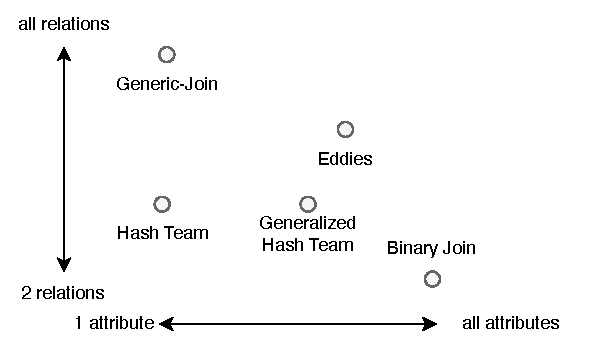
\includegraphics[width=.9\linewidth]{free-join.pdf}
  \caption{\FJ plans represent a design space of join algorithms
    that contains many existing algorithms.}
  \label{fig:free-join-space}
\end{figure}

\begin{figure*}
  \begin{subfigure}[t]{0.23\linewidth}
    \begin{lstlisting}
# [ R(x, y) | S(y) ]
# -> [ S(z) | T(z, x) ]

for (x,y) in R:
  s = S[y]? # S:y->[z]
  for z in s:
    if (z,x) in T:
      output(x,y,z)
\end{lstlisting}
    \caption{Plan equivalent to binary join.}
    \label{fig:bj-triangle}
  \end{subfigure}
  \begin{subfigure}[t]{0.25\linewidth}
    \begin{lstlisting}[numbers=none, showlines=true]
# [ R(x, y) | S(y), T(x) ]
# -> [ S(z) | T(z) ]

for (x,y) in R:
  s = S[y]?; t = T[x]?
  for z in s:
    if z in t:
      output(x,y,z)
\end{lstlisting}
    \caption{Another \FJ plan.}
    \label{fig:fj-triangle}
  \end{subfigure}
  \begin{subfigure}[t]{0.25\linewidth}
    \begin{lstlisting}[showlines=true]
# [ R(x, y) | S(y), T(x) ]
# -> [ S(z) $\cap$ T(z) ]

for (x,y) in R:
  s = S[y]?; t = T[x]?
  for z in s $\cap$ t:
    output(x,y,z)

\end{lstlisting}
    \caption{Plan with intersect ($\cap$).}
    \label{fig:inter-triangle}
  \end{subfigure}
  \begin{subfigure}[t]{0.25\linewidth}
    \begin{lstlisting}[showlines=true, numbers=none]
# [ R(y) $\cap$ S(y) ]
# -> [ S(z) $\cap$ T(z) ]
#    -> [ T(x) $\cap$ R(x) ]
for y in R.y $\cap$ S.y:
  for z in S[y] $\cap$ T.z:
    for x in T[z] $\cap$ R[y]:
      output(x,y,z)

\end{lstlisting}
    \caption{Plan equivalent to \GJ.}
    \label{fig:gj-triangle}
  \end{subfigure}
  \caption{Four different \FJ plans for $Q_\triangle$ and their execution.}
\end{figure*}

\subsection{Other Optimizations}\label{sec:other-optimizations}
In this section, we summarize a few additional optimizations
introduced in our SIGMOD paper~\cite{10.1145/3589295},
as well as relate \FJ to the \GJ algorithm.
To motivate these optimizations, we will follow the new example query
$Q_\triangle$ in Figure~\ref{fig:triangle-query}.
Note $Q_\triangle$ is now a {\em cyclic} query, because its hypergraph
is a triangle with three vertices $x$, $y$, and $z$ and three edges
corresponding to $R(x, y)$, $S(y,z)$, and $T(z, x)$.

Let us first consider the algorithm in Figure~\ref{fig:bj-triangle}.
We show the \FJ plan in the comments atop the figure,
and note that it is equivalent to binary join.
To reduce clutter we will stick with a row-wise notation
while keeping in mind the underlying columnar storage.
We also remove redudant values from the hash maps;
for example, the hash map for $S$ in Figure~\ref{fig:bj-triangle}
now maps every $y$ to a vector of $z$ (instead of a vector of $(y, z)$).
The binary join algorithm first iterates over $(x, y)$-tuples in $R$,
using each $y$ to probe into $S$ to get a vector of $z$.
For each $z$, it then probes into $T$ to check if $(z, x)$ is in $T$,
and outputs the tuple $(x, y, z)$ if so.
This binary plan essentially computes the join $R \bowtie S$ first
before discarding tuples that do not join with $T$.
Because $R\bowtie T$ has size $O(n^2)$,
the algorithm runs in quadratic time.
Since the relations are symmetric, any binary join plan
will have the same asymptotic run time.

A different algorithm is shown in Figure~\ref{fig:fj-triangle}.
Here, as we iterate over tuples in $R$, we look up into $S$ and $T$
at the same time.
In other words we perform the late iteration optimization again,
pulling up lookups to discard tuples early.
However, this is not sufficient, because every tuple in $R$
does in fact join with both $S$ and $T$,
so the first loop level discards no tuples.
As the second loop level iterates over $s$,
we are in effect still computing the join $R \bowtie S$
which takes $O(n^2)$ time.
To overcome this inefficiency, we now introduce a new operator
called {\em intersection} ($\cap$).

\subsubsection{Intersection}
In contrast, the algorithm in Figure~\ref{fig:inter-triangle}
runs in linear time.
The small difference is that we have replaced the inner loop of
Figure~\ref{fig:fj-triangle}, which iterates over $s$,
with a loop iterating over the intersection of $s$ and $t$.
When we compute the intersection, we always iterate over the smaller
set while probing into the larger set.
To analyze the run time of this algorithm,
we first assume we have built a hash map for $S$,
mapping each $y$ to a {\em hash set} of $z$,
and similar for $T$.
Building each hash map takes linear time.
Then, as we iterate over $R$, we consider three cases:
\begin{enumerate}
  \item For the tuple $(x_0, y_0)$, $s = S[y_0] = \setof{z_i}{i \in [0, \ldots, n]} = T[x_0] = t = s \cap t$,
        so we may iterate over either $s$ or $t$ to compute $s \cap t$ in linear time.
  \item For each tuple $(x_0, y_i)\mid i > 0$, $t = T[x_0] \setof{z_i}{i \in [0, \ldots, n]}$ but
        $s = S[y_i] = \set{z_0}$, so we iterate over (the only element of) $s$
        and probe into $t$ to compute $s \cap t$.
        This takes constant time for each $y_i$, so for all $y_i$ the total time is linear.
  \item The case for tuple $(x_i, y_0)$ is symmetric to the previous case, so it also takes linear time.
\end{enumerate}
Overall, the algorithm in Figure~\ref{fig:inter-triangle} runs in linear time.
Another way to think about the intersection operation is to
understand it as dynamically reording the iterations and lookups:
to compute $s \cap t$, we switch between
the plans $[S(z) \mid T(z)]$ and $[T(z)\mid S(z)]$ depending on which one is smaller.

\subsubsection{\GJ}
We can now faithfully derive the \GJ algorithm as a special case of \FJ,
using the itersection operator.
Suppose an instance of \GJ follows the variable order $x_1, x_2, \ldots, x_n$.
The corresponding \FJ plan is:
\begin{alignat*}{4}
   & [R_1^1(     &  & x_1) \cap R_1^2(x_1) \cap \cdots]                    \\
   & \rightarrow &  & [R_2^1(x_2) \cap R_2^2(x_2) \cap \cdots]             \\
   &             &  & \vdots                                               \\
   &             &  & \rightarrow [R_n^1(x_n) \cap R_n^2(x_n) \cap \cdots]
\end{alignat*}
where $R_i^j$ is a relation that contains $x_i$ in its schema.
When computing a multiway intersection, we (dynamically) pick
the smallest set to iterate over and probe into the rest.
For any choice of the variable order,
the \GJ algorithm is guaranteed to run in worst-case
optimal time~\cite{DBLP:conf/icdt/Veldhuizen14,DBLP:conf/pods/000118,DBLP:conf/pods/NgoPRR12}.


\subsubsection{Lazy trie building}
To explain the algorithm in Figure~\ref{fig:fj-triangle} we assumed
to have pre-built hash maps for $S$ and $T$.
A more efficient strategy is to {\em lazily} construct parts of the data structures
as we iterate over the relations.
Specifically, we will only build the hash set for $s$ (or $t$)
right before we need to probe into it.
This way, we can avoid building a linear number of (singleton) hash sets
that we only need to iterate over.
In the full paper~\cite{10.1145/3589295} we describe a data structure,
called Column-oriented Lazy Trie (COLT), that generalizes this idea.

\begin{figure}
  $Q_\triangle \cd R(x, y), S(y, z), T(z, x).$
  \begin{center}
    \begin{tabular}{c}
      \begin{lstlisting}[language=SQL, numbers=none]
SELECT * FROM R,S,T -- R(x,y), S(y,z), T(z,x)
 WHERE R.y = S.y AND S.z = T.z AND T.x = R.x
\end{lstlisting}
    \end{tabular}
  \end{center}
  \begin{align*}
    R  = \setof{(x_0, y_i)}{y \in [0 \ldots n]} \cup \setof{(x_i, y_0)}{y \in [0 \ldots n]} \\
    S  = \setof{(y_0, z_i)}{y \in [0 \ldots n]} \cup \setof{(y_i, z_0)}{y \in [0 \ldots n]} \\
    T  = \setof{(z_0, x_i)}{y \in [0 \ldots n]} \cup \setof{(z_i, x_0)}{y \in [0 \ldots n]}
  \end{align*}
  \caption{The triangle query $Q_\triangle$, and an input instance.}
  \label{fig:triangle-query}
\end{figure}

\begin{figure}
  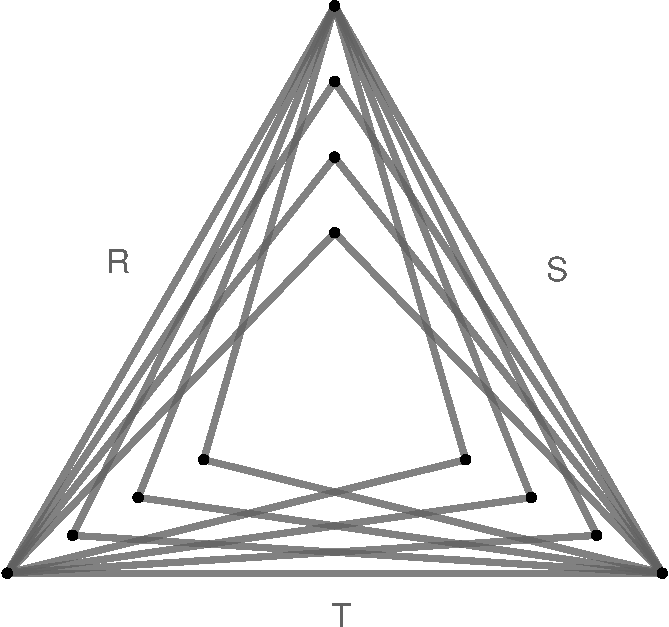
\includegraphics[width=.6\linewidth]{triangles-2.pdf}
  \caption{Visualization of input relations to $Q_\triangle$.
    Each relation is represented by a set of edges.
    The query $Q_\triangle$ looks for triangles formed by
    one edge from each relation (there are 10).}
\end{figure}

\begin{figure}
  \begin{lstlisting}
def join(plan, tuple, R, S, T, ...):
  if plan is empty: output(tuple)
  else:
    let [ R(xs) | S(ys), T(zs), ... ] = plan[0]
    for xs in R:
      r = R[xs]?; s = S[ys]?; t = T[zs]?; ...
      join(plan[1:], tuple ++ xs, r, s, t, ...)
\end{lstlisting}
  \caption{Recursive formulation of \FJ.}
  \label{fig:fj-recursive}
\end{figure}


\begin{figure}
  \begin{lstlisting}
def join(plan, tuple, R, S, T, ...):
  if plan is empty: output(tuple)
  else:
    let [ R(xs) | S(ys), T(zs), ... ] = plan[0]
    tup_rels = {} # map a partial tuple to sub-relations
    for xs_batch in R.iter_batch():
      for xs in xs_batch:
        r = R[xs]?; s = S[ys]?; t = T[zs]?; ...
        tup = tuple ++ xs
        tup_rels[tuple] = (r, s, t, ...)
    for (tup, rels) in tup_rels:
      join(plan[1:], tup, rels)
\end{lstlisting}
  \caption{Vectorized execution for \FJ.}
  \label{fig:vectorized-execution}
\end{figure}

\subsubsection{Vectorized Execution}\label{sec:vectorized-execution}
A simple way to implement \FJ is to use a recursive function,
as shown in Figure~\ref{fig:fj-recursive}.
For every group in the \FJ plan,
we iterate over the first subatom and probe into the remaining subatoms.
If all probes are successful, we append new values to the partial tuple,
and recursively call \lstinline|join| on the remaining plan and sub-relations.
This na\"ive implementation suffers from poor temporal locality:
in the body of the loop,
we probe into the same set of relations for each tuple.
But these probes are interrupted by the recursive
call at the end,
which is itself a loop interrupted by further recursive calls.

A simple way to improve locality is to perform a batch of probes
before recursing, just like the classic vectorized execution
for binary join.
As shown in Figure~\ref{fig:vectorized-execution},
we call \lstinline|iter_batch| to retrieve a batch of tuples from $R$.
For each tuple in a batch,
we probe into the relations to get the corresponding sub-relations.
If all probes are successful, we append new values to the partial tuple,
and pair the tuple with the respecitve sub-relations;
otherwise we continue onto the next tuple in the batch.
Finally, for each tuple that successfully probes into all relations,
we call \lstinline|join| recursively on the remaining plan.

% \subsection{\GJ}\label{sec:background:gj}

% \GJ was introduced in~\cite{DBLP:journals/sigmod/NgoRR13} and is the
% simplest worst-case optimal join algorithm.  It is based on the
% earlier Leapfrog Triejoin algorithm~\cite{DBLP:conf/icdt/Veldhuizen14}.
% %
% \GJ computes a join query through a series of nested
% loops, where each loop iterates over a {\em variable} (not a tuple).
% Concretely, \GJ chooses arbitrarily a variable $x$, computes the
% intersection of all $x$-columns of all relations containing $x$, and
% for each value $a$ in this intersection it computes the residual query
% $Q[a/x]$, where every relation $R$ that contains $x$ is replaced with
% $\sigma_{x=a}(R)$.  In pseudocode (where $\Pi_x (R_i)$ is the $x$-column of $R_i$):
% %
% \begin{lstlisting}[basicstyle=\ttfamily]
% def join(Q, tuple): # tuple is initially empty
%   if Q is empty: print(tuple)
%   else:
%     for a in $\bigcap_{i : x \in schema(R_i)} \Pi_x(R_i)$:
%       join(Q[a/x], tuple ++ [a])
% \end{lstlisting}
% %
% If the query $Q$ has $k$ variables, then there are $k$ nested loops in
% \GJ.  In the inner most loop, \GJ outputs the tuple of constants, one
% from each iteration.\footnote{For bag semantics, it multiplies their
%   multiplicities.}  We notice that a plan for \GJ consists of a total
% order of the variables of the query, which we denote as
% $[x_1, x_2, \ldots, x_k]$.  Assuming that the intersection above is
% done optimally (see below), the algorithm is provably
% worst-case-optimal, for any choice of the variable order.

% \begin{example}
%   Fig.~\ref{fig:background:gj} shows the execution of \GJ on the
%   query $Q_\triangle$, using the variable order $[x,y,z]$.  We denoted
%   $\Pi_x(R)$ by $R.x$, and denoted (with some abuse) $\sigma_{x=a}(R)$
%   by $R[a]$.
% \end{example}


% While binary joins use hash tables, an implementation of \GJ uses a
% \emph{hash trie}, one for each relation in the query.  The hash-trie
% is a tree, whose depth is equal to one plus the number of attributes
% of the relation, and where each node is either an empty leaf
% node,\footnote{For bag semantics, we store in the leaf the
%   multiplicity of the tuple.} or a hash map mapping each atomic value
% to another node.  We will call the \emph{level} of a node to be the
% distance from the root, i.e. the root has level 0, its children level
% 1, etc.  The hash-trie completely represents the relation: every
% root-to-leaf path corresponds precisely to one tuple in the relation.
% \GJ uses the hash-trie as follows.  In order to compute
% $\sigma_{x=a}(R)$, it simply probes the current hash table for the
% value $x=a$, and returns the corresponding child.  To compute an
% intersection $\Pi_x(R_1) \cap \Pi_x(R_2) \cap \cdots$, it selects the
% trie with the fewest keys, say $R_1$, then iterates over every value
% $a$ in the keys for $R_1$ and probes it in each of the hash-maps for
% $R_2, R_3, \ldots$; this is a provably optimal algorithm for the
% intersection.

% \begin{example}
%   Consider the query $Q_\triangle$ and the \GJ plan $[x, y, z]$.  We
%   first build a hash trie each for $R$, $S$, and $T$.  Each trie has
%   three levels including the leaf.  Level 0 of $R$ is keyed on $x$,
%   level 1 is keyed on $y$, level 2 contains empty leaf nodes, and
%   similarly for $S$ and $T$.  Consider again the pseudocode in
%   Figure~\ref{fig:background:gj}.  The first loop intersects level 0
%   of the $R$-trie and the $T$-trie.  For each value $a$ in the
%   intersection, we retrieve the corresponding children $R[a]$ and
%   $T[a]$ respectively; these are at level 1.  The second loop
%   intersects the hash map $R[a]$ (at level 1) with the level 0
%   hash-map of $S$.  For each value $b$ in the intersection it
%   retrieves the corresponding children (levels 2 and 1 respectively),
%   and, finally, the innermost loop intersects the $S$- and $T$-hash
%   maps (both at level 2), and outputs $(a,b,c)$ for each $c$ in the
%   intersection.  So far we have assumed set semantics; if the
%   relations have bag semantics, then we simply multiply the tuple
%   multiplicities on the leaves (level 3).
% \end{example}

% %%% The original \GJ algorithm was specified for set semantics,
% %%% however~\cite{DBLP:journals/pvldb/FreitagBSKN20} showed the algorithm
% %%% can be easily extended to bag semantics.  We therefore ignore the
% %%% difference between the two semantics for the rest of this paper.

% \subsection{Binary Join v.s. \GJ}
% Binary join and \GJ each have their own advantages and disadvantages.
% \GJ became popular because of its asymptotic performance guarantee:
% Ngo, R{\'{e}}, and Rudra~\cite{DBLP:journals/sigmod/NgoRR13} proved the algorithm is
% \emph{worst-case optimal} for \emph{any variable order}, in the sense
% that its run time is bounded by the largest possible size of its
% output, called AGM bound~\cite{DBLP:journals/siamcomp/AtseriasGM13}.
% For example, \GJ executes $Q_\triangle$ in time
% $\sqrt{|R|\cdot |S| \cdot |T|}$, which is $n^{3/2}$ when all relations
% have size $n$; in contrast, a binary join plan can take $\Omega(n^2)$.
% We note, however, that this formula does not include the preprocessing
% time needed to construct the tries.  For example, if $T$ is
% significantly larger than $R, S$, then the run time of \GJ is
% $\ll |T|$, yet during preprocessing \GJ needs to read the entire
% relation $T$.  On the other hand, binary join has been a staple of
% database systems for decades.  The hash table data structure is
% simpler than hash tries and is cheaper to build.  Techniques like
% vectorized execution and column-oriented layout have also made binary
% join practically efficient, but these optimizations have not been
% adapted for \GJ.  Binary join plans are known to be very sensitive to
% the choice of the optimizer: poor plans perform catastrophically
% bad~\cite{DBLP:journals/pvldb/LeisGMBK015}.  In contrast, although the
% runtime performance of \GJ does depend on the variable order, some
% researchers believe that \GJ is less sensitive to poor variable
% orders, in part because it is always theoretically optimal.


% %%% \subsection{Basic Concepts}\label{sec:basic-concepts}
% %%% 
% %%% First, we define relations under bag semantics:
% %%% 
% %%% \begin{definition}
% %%%   A \emph{relation} is a bag (multiset) of tuples.
% %%%   The number of values in a tuple is its \emph{arity}.
% %%%   Every tuple in the same relation has the same arity 
% %%%     which is also the arity of the relation.
% %%%   Each relation has a \emph{schema}, which is a tuple of distinct variables.
% %%%   The size of the schema is the same as the arity of the relation.
% %%% \end{definition}
% %%% 
% %%% For convenience, we sometimes refer to the schema of a tuple, 
% %%%   which is the schema of the relation holding that tuple.
% %%% We also associate each value in a tuple with a variable in the tuple's schema.
% %%% 
% %%% To simplify presentation we focus on queries involving only 
% %%%   natural joins in this paper, although our implementation 
% %%%   also supports standard relational algebra operations 
% %%%   like selection, projection and aggregation.
% %%% In other words, every query is a \emph{full conjunctive query}:
% %%% \begin{definition}
% %%%   A \emph{full conjunctive query} is a set of \emph{atom}s,
% %%%   where each atom is a relation name paired with a tuple of variables.
% %%%   The number of variables in each tuple is the same as the arity of the relation.
% %%%   We assume no two atoms share the same relation name, 
% %%%   and each variable appears at most once in the same atom.
% %%% \end{definition}
% %%% 
% %%% We handle a self-join of a relation $R$
% %%%   by creating a copy of $R$ and renaming it to $R'$.
% %%% This is the standard approach in database systems 
% %%%   that require each query plan to be a tree.
% %%% Without loss of generality,
% %%%   we assume each relation's schema coincides with 
% %%%   the variables of its atom in the query.
% %%% 
% %%% \begin{example}
% %%%   Consider the \emph{triangle query} over relations $R$, $S$, $T$:
% %%% $$Q_{\triangle} \cd R(x, y), S(y,z), T(x, z).$$
% %%% It is the same as the following SQL query:
% %%% \begin{lstlisting}[
% %%%     language=SQL,
% %%%     showspaces=false,
% %%%     basicstyle=\ttfamily\small,
% %%%     numbers=left,
% %%%     numberstyle=\tiny,
% %%%     commentstyle=\color{gray}
% %%%  ]
% %%% SELECT * FROM R, S, T -- schema: R(x,y), S(y,z), T(x,z)
% %%%  WHERE R.y = S.y AND S.z = T.z AND T.x = R.x
% %%% \end{lstlisting}
% %%% \end{example}
% %%% 
% %%% The precise definition of cyclic and acyclic queries 
% %%%   is not important for this paper,
% %%%   so we discuss them informally and briefly here.
% %%% Fix a conjunctive query $Q$.
% %%% The \emph{query hypergraph} of $Q$ consists of vertices $\mathcal{V}$
% %%%   and edges $\mathcal{E}$, 
% %%%   where each $v \in \mathcal{V}$ is a variable
% %%%   and each hyperedge $(v_1, \ldots, v_k) \in \mathcal{E}$
% %%%   is the relation whose atom has the variables $(v_1, \ldots, v_k)$.
% %%% A sufficient condition for a query to be acyclic is that 
% %%%   the query hypergraph is a tree.
% %%% $Q_\triangle$ is a \emph{cyclic} query, 
% %%%   whereas any chain query is acyclic, e.g. $Q \cd R(x,y), S(y, z), T(z,w).$
% %%% 
% %%% \subsection{Binary Join}\label{sec:binary-join}
% %%% Now we review relevant concepts for binary join, 
% %%%   including its data structures, query plan.
% %%% 
% %%% Binary join works over \emph{hash tables}:
% %%% 
% %%% \begin{definition}
% %%%   A \emph{hash table} for $R$ is a hash map where each key is a tuple, 
% %%%     and every key is mapped to a vector of tuples.
% %%% \end{definition}
% %%% 
% %%% A \emph{binary plan} specifies how to execute a query with binary join:
% %%% 
% %%% \begin{definition}
% %%%   A \emph{binary plan} is a binary tree where each leaf is a distinct relation.
% %%%   A \emph{left-deep linear plan} is a binary plan where every right-child of an internal node is a leaf.
% %%%   Alternatively, we can write every left-deep linear plan as a sequence of relation names.
% %%%   There is a unique leaf that is a left-child, and the relation of that leaf is called the \emph{left relation}.
% %%%   A binary plan that is not a left-deep linear plan is called a \emph{bushy plan}.
% %%% \end{definition}
% %%% 
% %%% By this definition, we consider both ``right-deep'' plans and ``zig-zag'' plans as bushy plans,
% %%%   and do not distinguish between them.
% %%% A standard relational database executes a bushy plan by decomposing it into a series of left-deep linear plans.
% %%% That is, for each leaf on the left, it traverses the binary tree bottom-up by going only to the left parent,
% %%%   and all the nodes visited form a left-deep linear plan.
% %%% Then we execute these plans starting with the right-most one, materializing the intermediate results as we go.
% %%% We omit a formal description of this process for brevity.
% %%% Our system decomposes bushy plans in exactly the same way,
% %%%   and we will focus on left-deep linear plans in the rest of this paper.
% %%% 
% %%% \begin{example}
% %%%   A possible left-deep linear plan for $Q_\triangle$ is $[R, S, T]$.
% %%% \end{example}
% %%% 
% %%% We assume the reader is familiar with how a left-deep linear plan executes,
% %%%   and only provide an informal example here.
% %%%   of binary join for a different query.
% %%% 
% %%% \begin{figure}
% %%%   \begin{subfigure}[b]{0.45\linewidth}
% %%% \begin{lstlisting}
% %%% for (x, y) in R:
% %%%   S = S[y]?
% %%%   for z in S:
% %%%     T = T[x,z]?
% %%%     for () in T:
% %%%       output(x, y, z)
% %%% \end{lstlisting}
% %%%     \caption{Binary join.}
% %%%     \label{fig:back-binary-join}
% %%%   \end{subfigure}
% %%%   \begin{subfigure}[b]{0.45\linewidth}
% %%%     \centering
% %%% \begin{lstlisting}
% %%% for x in R.x $\cap$ T.x:
% %%%   R = R[x]; T = T[x]
% %%%   for y in R.y $\cap$ S.y:
% %%%     S = S[y]
% %%%     for z in S.z $\cap$ T.z:
% %%%       output(x, y, z)
% %%% \end{lstlisting}
% %%%     \caption{\GJ.}
% %%%     \label{fig:back-gj}
% %%%   \end{subfigure}
% %%%   \Description[TODO]{TODO}
% %%%   \caption{Execution of binary join and \GJ for $Q_\triangle$.
% %%%   The notation \lstinline|S[y]?| performs a lookup on $S$ with the key $y$,
% %%%    and continues to the enclosing loop if the lookup fails.  }
% %%% \end{figure}
% %%% 
% %%% \begin{example}
% %%%   Given the query $Q_\triangle$ and the plan $[R, S, T]$,
% %%%     we first build a hash table for $S$ keyed on $y$,
% %%%     where each $y$ maps to a vector of $z$ values.
% %%%     Then we build a hash table for $T$ keyed on $x$ and $z$,
% %%%     each mapped to a vector of empty tuples\footnote{
% %%%       We store the vectors of empty tuples to enforce bag semantics.
% %%%       An efficient implementation may simply store a count of duplicates.
% %%%     }.
% %%%   The nested loops in Figure~\ref{fig:back-binary-join} show the execution 
% %%%     of binary join.
% %%%   For each tuple $t = (x, y)$ in $R$, 
% %%%     we first probe into the hash table for $S$ using $y$
% %%%     to get a vector of $z$ values.
% %%%   We then loop over each $z$ 
% %%%     and probe into the hash table for $T$ using $x$ and $z$. 
% %%%   Each successful probe will return a vector of empty tuples, 
% %%%     and we output the tuple $(x, y, z)$ for each empty tuple.
% %%% \end{example}
% %%% 
% %%% \subsection{\GJ}
% %%% This section reviews basics of \GJ,
% %%%   including the hash trie data structure, 
% %%%   the \GJ plan, 
% %%%   and the execution of \GJ.
% %%% 
% %%% The data structure \GJ uses is called the \emph{hash trie}, 
% %%%   defined recursively as follows:
% %%% 
% %%% \begin{definition}
% %%%   A \emph{hash trie} is either a leaf, 
% %%%     or a hash map where each key is a single value 
% %%%       and every key is mapped to a hash trie.
% %%% \end{definition}
% %%% 
% %%% A hash trie can be seen as a tree, where 
% %%%   the concepts of \emph{parent}, and \emph{child}
% %%%   are defined in the usual way.
% %%% 
% %%% \begin{definition}
% %%%  A trie is a \emph{root} if it has no parents;
% %%%   any trie that is not a root is a \emph{subtrie}.
% %%% The \emph{level} of a subtrie is its distance from the root,
% %%%   i.e., the root is at level 0.
% %%% \end{definition}
% %%% 
% %%% A trie can represent a relation, 
% %%%   where the $i$-th level of the trie 
% %%%   stores values of the $i$-th attribute of the relation.
% %%% All the values along each path from the root to a leaf form 
% %%%   a tuple in the relation.
% %%% 
% %%% Now we define the \GJ plan that specify how to execute a query with \GJ.
% %%% 
% %%% \begin{definition}
% %%%   Fix a query $Q$.
% %%%   A \GJ plan for $Q$ is a total ordering of the variables in $Q$.
% %%% \end{definition}
% %%% 
% %%% A \GJ plan is executed by a series of nested loops, 
% %%%   where each loop level processes one variable 
% %%%   by \emph{intersecting} multiple tries on that variable.
% %%% We omit a formal definition for brevity, 
% %%%   and instead provide an informal example.
% %%% 
% %%% \begin{example}
% %%%   Consider the query $Q_\triangle$ and the \GJ plan $[x, y, z]$.
% %%%   We first build a hash trie each for $R$, $S$, and $T$.
% %%%   Each trie has three levels including the leaf.
% %%%   The first two levels for $R$, $S$, and $T$ are 
% %%%     keyed on $(x,y)$, $(y,z)$, and $(x,z)$, respectively.
% %%%   The execution of \GJ over these tries is shown in Figure~\ref{fig:back-gj}.
% %%%   The first loop intersects the tries for $R$ and $T$ on their keys.
% %%%   For each value $x$ in the intersection, 
% %%%     we retrieve the subtries mapped to $x$ from $R$ and $T$ respectively.
% %%%   The second loop intersects the subtrie for $R$ with the trie for $S$ on $y$,
% %%%     and retrieves the subtrie mapped to $y$ from $S$.
% %%%   Finally, the innermost loop intersects the subtries for $S$ and $T$ on $z$,
% %%%     and outputs the tuple $(x, y, z)$ for each value $z$ in the intersection.
% %%% \end{example}
% %%% 
% %%% The original \GJ algorithm was specified for set semantics, 
% %%%   however~\cite{DBLP:journals/pvldb/FreitagBSKN20} showed
% %%%   the algorithm can be easily extended to bag semantics.
% %%% We therefore ignore the difference between the two semantics 
% %%%   for the rest of this paper.
% %%% 
% %%% \subsection{Binary Join v.s. \GJ}
% %%% Binary join and \GJ each have their own advantages and disadvantages.
% %%% \GJ became popular because of its asymptotic performance guarantee:
% %%%   \citet{DBLP:journals/sigmod/NgoRR13} proved the algorithm is 
% %%%   \emph{worst-case optimal}, in the sense that 
% %%%   its run time is bounded by the worst-case output size.
% %%% For example, if each of the three relations in $Q_\triangle$ has $n$ tuples,
% %%%   there can be at most $n^{3/2}$ tuples in the output, 
% %%%   and \GJ runs in $O(n^{3/2})$ time.
% %%% In contrast, a binary join plan can take $\Omega(n^2)$ time 
% %%%   to compute the same query.
% %%% On the other hand, binary join has been a staple of database systems for decades. 
% %%% The hash table data structure is simpler than hash tries and is cheaper to build.
% %%% Techniques like vectorized execution and column-oriented layout have also 
% %%%   made binary join practically efficient,
% %%%   but these optimizations have not been adapted for \GJ.
% %%% 
\section{From binary join to \FJ}\label{sec:free-join}

\subsection{Binary Join}

% We start by presenting the Generalized Hash Trie (\GHT) which
% is the data structure used in \FJ (Section~\ref{sec:ght}).
% Next we introduce the \FJ plan that specifies
% how to execute a query with \FJ (Section~\ref{sec:fj-plan}).
% Finally, we describe the \FJ algorithm,
% which takes as input a collection of \GHTs
% and a \FJ plan,
% and computes the query according to the plan (Section~\ref{sec:free-join-algorithm}).

% We will show how each of the above components generalizes
% and unifies the corresponding components in binary join
% and \GJ:
% the \GHT generalizes hash tables and hash tries,
% the \FJ plan generalizes binary plans and \GJ plans, and
% the \FJ algorithm generalizes binary join and \GJ.


\subsection{The Generalized Hash Trie}\label{sec:ght}

\begin{figure}
  \begin{lstlisting}
interface GHT {
  # fields
  relation: String, vars: Vec<String>  
  # constructor
  fn new(name: String, schema: Vec<Vec<String>>) -> Self
  # methods
  fn iter() -> Iterator<Tuple>
  fn get(key: Tuple) -> Option<GHT> }
\end{lstlisting}
  \caption{The \GHT interface.}
  \label{fig:ght}
\end{figure}

To unify binary join and \GJ,
we first need to unify the data structures they work over.
We propose the Generalized Hash Trie
which generalizes both the hash table used in binary join
and the hash trie used in \GJ.

\begin{definition}[Generalized Hash Trie (\GHT)]
  A \GHT is a tree where each leaf is a vector of tuples, and
  each internal node is a hash map whose keys are tuples, and each key
  maps to a child node.
\end{definition}

We will reuse the terminology defined for tries, including
\emph{level}, \emph{node}, and \emph{leaf}, etc., for \GHTs.  We will
also use the terms \GHT and \emph{trie} interchangeably when the
context is clear.  The {\em schema} of a \GHT is the list
$[\bm y_0,\bm y_1, \ldots, \bm y_\ell]$ where $\bm y_k$ are the
attribute names of the key at level $k$.

The hash trie used in \GJ is a \GHT where each key is a tuple of size one,
and the last level stores empty vectors, each of which represents a leaf.
The hash table used in binary join is very similar to a \GHT with only two levels,
where level 0 stores the keys and level 1 stores
vectors of tuples.
A small difference is that, in the \GHT, the concatenation of
a tuple from level 0 with a tuple from level 1 forms a tuple in the relation,
whereas each whole tuple is stored directly in a hash table.
We will show in Section~\ref{sec:colt} how the \COLT data structure
more faithfully captures the structure of a hash table.
Figure~\ref{fig:ght-examples} shows two examples of \GHTs.

We use \GHTs to represent relations,
and attach metadata as well as access methods
to each \GHT, to be used by the \FJ algorithm.
The \GHT interface is shown in Figure~\ref{fig:ght}.
The \lstinline|relation| field stores the relation name.
A sub-trie inherits its name from its parent.
The \lstinline|vars| field stores parts of the relation's schema:
if the trie is a vector of tuples,
\lstinline|vars| is the schema of each tuple;
if the trie is a map,
\lstinline|vars| is the schema of each key.
The constructor method \lstinline|new| creates a new \GHT from the named relation,
where an $n$-th level trie has variables
matching the $n$-th element of the \lstinline|schema| argument,
and the values along each path from the root to a leaf of the \GHT
form a tuple in the relation.

\begin{example}
  Both \GHTs in Figure~\ref{fig:ght-examples} represent relation $S$ from the
  clover query $Q_\clubsuit$ in Figure~\ref{fig:clover-query}.  The
  \GHT on the left (a hash trie) was created by calling the
  constructor method \lstinline|new| with the schema
  \lstinline|[[x],[b],[]]|, so the top-level trie has the schema
  \lstinline|[x]|, each second-level trie has the schema
  \lstinline|[b]|, and each third-level trie (a leaf) has the empty
  schema \lstinline|[]|.  The \GHT on the right (a hash table) was
  created by calling \lstinline|new| with the schema
  \lstinline|[[x],[b]]|.  It has only two levels, with schema
  \lstinline|[x]| and \lstinline|[b]|, respectively.  Note that each
  $b$ value in the hash trie is hashed and stored as a key, while the
  $b$ values in the hash table are simply stored in vectors.
\end{example}

The methods \lstinline|iter| and \lstinline|get|
provide access to values stored in the trie.
If the trie is a map,
\lstinline|get(key)| returns the sub-trie mapped to \lstinline|key|,
if any.
Calling \texttt{get} on a vector returns \lstinline|None|.
If the trie is a vector,
\lstinline|iter()|
returns an iterator over the tuples in the vector;
calling \texttt{iter} on a map
returns an iterator over the keys.

\begin{figure}
  \centering
  \begin{subfigure}[c]{0.3\linewidth}
    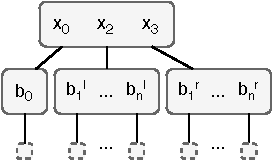
\includegraphics[width=\textwidth]{trie}
  \end{subfigure}\hspace{1.5cm}%
  \begin{subfigure}[c]{0.3\linewidth}
    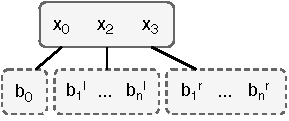
\includegraphics[width=\textwidth]{map}
  \end{subfigure}
  \caption{
    Two \GHTs. The one on the left is also a hash trie,
    and the one on the right is similar to a hash table.
    Each box with solid border stores hash keys,
    and each box with dashed border is a vector of tuples.
    An empty box is an empty vector, representing a leaf.
  }
  \label{fig:ght-examples}
\end{figure}

\begin{example}
  On the second \GHT in Figure~\ref{fig:ght-examples},
  calling \texttt{iter} returns an
  iterator over the values $[x_0, x_2, x_3]$.
  Calling \texttt{get} with the key $x_2$
  returns the sub-trie which is the vector $[b_1^l, \ldots, b_n^l]$.
  Calling \texttt{iter} on this sub-trie
  returns an iterator over $[b_1^l, \ldots, b_n^l]$.
\end{example}


\subsection{The \FJ plan}\label{sec:fj-plan}

% \ds{The section tile doesn't seem right.  What about ``The \FJ plan''}

A \FJ plan specifies how the \FJ algorithm should be executed.
It generalizes and unifies binary join plans and \GJ plans.
Recall that a left-deep linear plan for binary join
is a sequence of relations;
it need not specify the join attributes,
since all shared attributes are joined.
In contrast, a \GJ plan is a sequence of variables;
it need not specify the relations,
since all relations on each variable are joined.
A \FJ plan may join on any number of variables and relations at each step,
and therefore needs to specify both explicitly.

To help define the \FJ plan, we introduce two new concepts, called
\emph{subatom} and \emph{partitioning}.  Fix the query $Q$ in
Eq.~\eqref{eq:cq}:

\begin{definition}
  A \emph{subatom} of an atom $R_i(\bm x_i)$ is an expression
  $R_i(\bm y)$ where $\bm y$ is a subset of the variables $\bm x_i$.
  A \emph{partitioning} of the atom $R_i(\bm x_i)$ is a set of
  subatoms $R_i(\bm y_1), R_i(\bm y_2), \ldots$ such that
  $\bm y_1, \bm y_2, \ldots$ are a partition of $\bm x_i$.
\end{definition}

We now define the \FJ plan using these concepts.

\begin{definition}[\FJ Plan]
  Fix a conjunctive query $Q$.  A \FJ \emph{plan} is a list
  $[\phi_1, \ldots, \phi_m]$, where each $\phi_k$ is a list of
  subatoms of $Q$, called a {\em node}.  The nodes are required to
    {\em partition the query}, in the sense that, for every atom
  $R_i(\bm x_i)$ in the query, the set of all its subatoms occurring
  in all nodes must form a partitioning of $R_i(\bm x_i)$.  We denote
  by $vs(\phi_k)$ the set of variables in all subatoms of $\phi_k$.
  The variables \emph{available to} $\phi_k$ are all variables of the
  preceding nodes:
  %
  $$avs(\phi_k) = \bigcup_{j < k} vs(\phi_j)$$
  %
\end{definition}

%%% Since the partitioning of each atom into subatoms can be inferred 
%%%   from the sequence of nodes, we will omit the partitioning 
%%%   when specifying a \FJ plan.

We will define shortly a {\em valid plan}, but first we show an example.

%%% While a \GJ plan consists of total order of the variables, a \FJ plan
%%% defines only a partial order, if we set
%%% $vs(\Phi_i) < vs(\Phi_2) < \cdots$.


\begin{example}\label{ex:fj-plan}
  The following is an \FJ plan for $Q_\clubsuit$:
  \begin{align}
     & [[R(x, a), S(x)], [S(b), T(x)], [T(c)]]\label{eq:bj-plan}
  \end{align}
  %
  To execute the first node we iterate over each tuple $(x, a)$ in $R$
  and use $x$ to probe into $S$; for each successful probe we execute
  the second node: we iterate over each $b$ in $S[x]$, then use
  $x$ to probe into $T$; finally the third node iterates over $c$ in
  $T[x]$.  The reader may notice that this corresponds precisely to the
  left-deep plan $(R(x,a) \Join S(x,b))\Join T(x,c)$.
  %
  Another \FJ plan for $Q_\clubsuit$ is:
  %
  \begin{align}
    [[R(x), S(x), T(x)], [R(a)], [S(b)], [T(c)]]\label{eq:gj-plan}
  \end{align}
  %
  This plan corresponds to the \GJ plan $[x,a,b,c]$.  Intuitively, here
  we start by intersecting $R.x \cap S.x \cap T.x$, then, for each $x$
  in the intersection, we retrieve the values of $a$, $b$, and $c$ from
  $R$, $S$, and $T$, and output their Cartesian product.
\end{example}

% \begin{figure}
%   \begin{subfigure}[t]{0.4\linewidth}
%     \centering
%     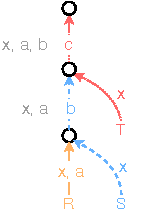
\includegraphics[height=35mm]{fj.pdf}
%     \caption{Plan in Eq.~\eqref{eq:bj-plan} (binary)}
%     \Description[TODO]{TODO}
%     \label{fig:bj-plan}
%   \end{subfigure}
%   \begin{subfigure}[t]{0.5\linewidth}
%     \centering
%     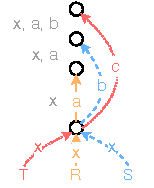
\includegraphics[height=32mm]{gj.pdf}
%     \caption{Plan in Eq.~\eqref{eq:gj-plan} (\GJ)}
%     \label{fig:gj-plan}
%   \end{subfigure}
%   \caption{Visualization of \FJ plans using notations from tensor
%     algebra~\cite{DBLP:journals/pacmpl/KjolstadKCLA17}.  Each circle
%     is a join node.  Arrows pointing to a node indicate the subatoms
%     in that node.  The same color and line style signify the same
%     relation. Grey text shows available variables.}
%   \label{fig:fj-plans}
% \end{figure}

% Readers familiar with tensor algebras may view \FJ as an
% \emph{iteration graph}~\cite{DBLP:journals/pacmpl/KjolstadKCLA17}, as
% shown in Figure~\ref{fig:fj-plans}.  We can ``read off'' the binary
% join plan $[R, S, T]$ from Figure~\ref{fig:bj-plan} by ignoring the
% variables.  Similarly, if we follow the variables in
% Figure~\ref{fig:gj-plan} bottom-up and ignore duplicates, we obtain the \GJ
% plan $[x, a, b, c]$.

Not all \FJ plans are valid, and only valid plans can be executed.  We
execute each \FJ node by iterating over one relation in that node, and
probe into the others.  Therefore, the values used in each probe must
be available, either from the same node or a previous one.

\begin{definition}
  A \FJ plan is \emph{valid} if for every node $\phi_k$ the following
  two properties hold.  (a) No two subatoms share the same relation,
  and (b) there is a subatom containing all variables in
  $vs(\phi_k) - avs(\phi_k)$.  We call such an subatom a \emph{cover}
  for $\phi_k$, and write $cover(\phi_k)$ for the set of covers.
\end{definition}

We will assume only valid plans in the rest of the paper.  To simplify
the presentation, in this section we assume that each node $\Phi_k$,
has {\em one} subatom designated as cover, and will always list it as
the first subatom in $\Phi_k$.  We will revisit this assumption in
Sec.~\ref{sec:optimization}, and allow for multiple covers.

%%% By this definition, every node must contain at least one subatom.  In
%%% addition, since we rename relations in a self-join as described in
%%% Section~\ref{sec:background}, a variable cannot appear in more than
%%% one subatom with the same relation name, and the same variable cannot
%%% appear more than once in the same subatom.

\begin{example}
  Both plans in Example~\ref{ex:fj-plan} are valid.  The covers for
  the 3 nodes for Eq.~\eqref{eq:bj-plan} are $R(x, a)$, $S(b)$, and
  $T(c)$, respectively. For the plan in Eq.~\eqref{eq:gj-plan}, the
  covers for the 4 nodes are $R(x), R(a), S(b), T(c)$; for the first
  node we could have also chosen $S(x)$ or $T(x)$ as cover.
\end{example}

% \ds{A few issues in the paragraph above and earlier.  You need to
%   define an atom, since this seems to be nonstandard: I assume you
%   mean that an atom consists of a relation name and a subset of the
%   variables.  The statement ``we do not allow self-joins'' raises
%   eyebrows; I don't think you mean that, please clarify.  The last
%   restriction (no atom contains the same variable twice) is OK, but
%   should be stated and explained in Sec.~\ref{sec:background}.}
% \rw{Will clarify in Backgroud.
%  For self-joins, we do allow them, but we rename the relation names to be different,
%  so that it looks like a join between different relations.
%  I'll also clarify this in Backgroud.  }
% \rw{Add because we rename them.}
% \rw{Use partial atom instead of an atom.}

% \ds{Before the next example add a brief explanation why the plans in
%   Ex.~\ref{ex:fj-plan} are valid.}
\begin{example}
  An example of an \emph{invalid} plan for the clover query has one
  single node containing all relations and variables:
  %
  $$[[R(x, a), S(x, b), T(x, c)]]$$
  %
  Intuitively, we cannot execute it: if we iterate over, say $R$, then
  we bind two variables $x$ and $a$, but to lookup $S$ we
  need the key $(x,b)$.
\end{example}

% \rw{We partition each atom to subatoms, 
% and define a plan for the query.
% }
% \begin{definition}
%   Given a \FJ plan $[\phi_1, \ldots, \phi_n]$, where 
% $\phi_i = \set{R_1(\overline{x_{i,1}}), \ldots, R_m(\overline{x_{i,m}})}$,
% \FJ computes the query:
% $$Q(*) \cd R_1(\overline{x_{1,1}}, \ldots, \overline{x_{n,1}}), \ldots, R_m(\overline{x_{1,m}}, \ldots, \overline{x_{n,m}}).$$
% That is, for each relation, we concatenate all its variables in the plan in order to form the query. 
% \end{definition}

% \begin{example}
%   Both plans in Eq.~\eqref{eq:bj-plan} and Eq.~\eqref{eq:gj-plan} 
%   compute the clover query $Q(x,a,b,c) \cd R(x,a), S(x,b), T(x,c).$
% \end{example}

% \ds{Add a definition saying ``Given a plan $P$, the query computed by
%   $P$ is $\ldots$'' Then illustrate this defintion with
%   Example~\ref{ex:fj-plan} and the example below.}

% \begin{example}
%   The plan $[\phi=\set{R(), S(), T()}]$ is valid and computes the three-way 
%   Cartesian product of the relations (it does not compute the clover query).
%   The plan is vacuously valid because $vs(\phi) = \emptyset$.
%   Both plans in Eq.~\eqref{eq:bj-plan} and Eq.~\eqref{eq:gj-plan} are also valid.
% \end{example}

% \ds{Equation numbers should be referred to using $\backslash$eqref
%   instead of $\backslash$ref.  I changed them in this file.}

\subsection{Execution of the \FJ Plan}\label{sec:free-join-algorithm}

% \ds{Suggestion: I would call this section ``Execution of the \FJ
%   Plan'' to better connect it to the previous section.}

The execution of a \FJ plan has two phases: the build phase and the
join phase.  The build phase constructs the \GHTs for the relations in
the query, by calling the constructor method \lstinline|new| on each
relation with the appropriate schema.  The join phase works over the
\GHTs to compute the join of the relations.

% fn ght_schema(relation, plan):
%   schema = []
%   for node in plan:
%     for atom in node:
%       if atom.relation == relation:
%         schema.append(atom.variables)
%   return schema 

\begin{figure}
  \begin{lstlisting}[
    commentstyle=\color{gray},
    escapeinside={(*}{*)},
    ]
fn join(all_tries, plan, tuple):
  if plan == []:
    output(tuple) (* \label{lst:output} *)
  else:
    tries = [ t $\in$ all_tries | t.relation $\in$ plan[0] ] (* \label{lst:select} *)
    # iterate over the cover
    @outer for t in tries[0].iter(): (* \label{lst:outer} *)
      subtries = [ iter_r.get(t) ] (* \label{lst:inner} *)
      tup = tuple + t
      # probe into other tries
      for trie in tries[1..]:     
        key = tup[trie.vars] (* \label{lst:key} *)
        subtrie = trie.get(key)
        if subtrie == None: continue @outer
        subtries.push(subtrie) (* \label{lst:inner-end} *)
      new_tries = all_tries[tries $\mapsto$ subtries] (* \label{lst:tuple} *)
      join(new_tries, plan[1:], tup) (* \label{lst:join} *)
\end{lstlisting}
  \caption{The \FJ algorithm.}
  \label{fig:fj-algo}
\end{figure}

\subsubsection*{Build Phase}
The build phase constructs a \GHT for each relation (atom)
$R_i(\bm x_i)$, as follows.  If the plan partitions the atom into the
subatoms $R_i(\bm y_0), R_i(\bm y_1), \ldots, R_i(\bm y_{\ell-1})$,
then the schema of its \GHT is the list
$[\bm y_0, \bm y_1, \ldots, \bm y_{\ell-1}, []]$.  Recall that the
last level of a \GHT is a vector instead of a hash map. As an
optimization, if the last subatom $R_i(\bm y_{\ell-1})$ is the cover
of its node, then we drop the last $[]$ from the schema, in other
words, we construct a vector for the $\bm y_{\ell-1}$.  After
computing the schema for each relation, we call the constructor method
\lstinline|new| on each relation and its computed schema to build the
\GHTs.

\begin{example}
  Consider the plan in Eq.~\eqref{eq:bj-plan} for the clover query
  $Q_\clubsuit$.  The \GHT schemas for $R$, $S$, and $T$ are
  $[[x, a]]$, $[[x], [b]]$, and $[[x], [c]]$ respectively.  Thus, $R$
  is a flat vector of tuples, and each of $S$ and $T$ is a hash map of
  vectors of values.  Consider now the triangle query $Q_{\triangle}$
  and the plan $[[R(x,y),S(y),T(x)],[S(z),T(z)]]$.  The \GHT
  schemas for $R, S, T$ are $[[x,y]]$, $[[y],[z]]$, and $[[x],[z],[]]$:
  in other words $R$ is stored as a vector, $S$ is a hash-map of
  vectors, and $T$ is a hash-map of hash-maps of vectors.
\end{example}

\subsubsection*{Join Phase}
The pseudo-code for the \FJ algorithm is shown in Figure~\ref{fig:fj-algo}.
The \lstinline|join| method takes as input the \GHTs, the \FJ plan,
and the current tuple initialized to be empty.
If the plan is empty, we output the tuple (line~\ref{lst:output}).
Otherwise, we work on the first node in the plan
and intersect relevant tries (line~\ref{lst:select}).
We iterate over tuples in the covering relation,
which is the first trie in the node (line~\ref{lst:outer}).
%
% First we pick the trie to iterate over (line~\ref{lst:iter}).
% If any trie is a vector, we iterate over it.
% % \dan{I think it's clearer if you always iterate over the first
% %   subatom, which is the cover of the node.  We just need to make sure
% %   that this subatom is a vector, when that's possible.}
% % For now, we assume for each join node, at most one trie is a vector.
% % %
% % \yell{At this point there is nothing left to assume.  The \GHT is well
% %   defined, and only its last level is a vector, and the \GHT schema
% %   for a plan is well defined.  Everything is well defined.}
% % %
% We will relax this assumption in Section~\ref{sec:colt}.
% If all tries are hash maps, we iterate over the one with the fewest keys.
% After picking the trie to iterate over, 
%   we sort the other tries by some estimated cost to probe into them (line~\ref{lst:probe}).
% For example, we can probe into the smaller trie first, 
%   since it is likely to be selective, and may fit into the cache.
%
% In the outer for loop (line~\ref{lst:outer})
%   we iterate over each tuple \lstinline|t| in the trie we have picked.
Then, we use values from \lstinline|t|
and the \lstinline|tuple| argument
as keys to probe into the other tries
(line~\ref{lst:inner}-\ref{lst:inner-end}).
To construct a key for a certain trie,
we find the values mapped from the trie's schema variables
in \lstinline|t| and \lstinline|tuple| (line~\ref{lst:key}).
If any probe fails, we continue to the next tuple in the outer loop.
If all probes succeed, we replace the original tries with the
subtries returned by the probes,
and recursively call \lstinline|join|
on the new tries and the rest of the plan (line~\ref{lst:tuple}-\ref{lst:join}).

The recursive definition may obscure the essence of the \FJ algorithm,
so we provide some examples where we unroll the recursion.
We introduce some convenient syntax to simplify the presentation.
We write \lstinline|for (x,y,...) in T:|
to introduce a for-loop iterating over \lstinline|T|,
binding the values of each tuple in \lstinline|T.iter()|
to the variables \lstinline|x,y,...|.
We write \lstinline|r = R[t]?| to bind the result of
\lstinline|R.get(t)| to \lstinline|r|;
if the lookup fails, we continue to the next iteration of the
enclosing loop.
In other words, \texttt{r = R[t]?} is equivalent to:
%
\begin{lstlisting}
r = R.get(t); if r.is_none(): continue
\end{lstlisting}

% \begin{figure*}
%   \begin{subfigure}[b]{0.3\linewidth}
%     \begin{lstlisting}[escapeinside={(*}{*)}]
% R = GHT("R",[["x","a"]])
% S = GHT("S",[["x"],["b"]])
% T = GHT("T",[["x"],["c"]])
% for (x, a) in R:
%   s = S[x]?
%   for b in s:
%    (* \underline{t = T[x]?} *)
%     for c in t:
%       output(x, a, b, c)
% \end{lstlisting}
%     \caption{Binary \FJ.}
%     \label{fig:bj-loop}
%   \end{subfigure}
%   \hspace{1.5em}
%   \begin{subfigure}[b]{0.3\linewidth}
%     \centering
%     \begin{lstlisting}[
%     escapeinside={(*}{*)}
% ]
% # same as the left
% # ...
% # ...
% for (x, a) in R:
%   s = S[x]?
%  (* \underline{t = T[x]?} *)
%   for b in s:
%     for c in t:
%       output(x, a, b, c)
% \end{lstlisting}
%     \caption{Factorized \FJ.}
%     \label{fig:factorized-loop}
%   \end{subfigure}
%   \hspace{.5em}
%   \begin{subfigure}[b]{0.3\linewidth}
%     \centering
%     \begin{lstlisting}
% R = GHT("R",[["x"],["a"]])
% # same as the left
% # ...
% for x in R:
%   r=R[x]?; s=S[x]?; t=T[x]?
%   for a in r:
%     for b in s:
%       for c in t:
%         output(x, a, b, c)
% \end{lstlisting}
%     \caption{Generic \FJ.}
%     \label{fig:gj-loop}
%   \end{subfigure}
%   \caption{Execution of \FJ for the clover query.}
% \end{figure*}

\begin{example}\label{ex:binary-free-join}
  Consider the plan in Eq.~\eqref{eq:bj-plan} for the clover query $Q_\clubsuit$.
  Figure~\ref{fig:bj-loop} shows its execution; ignore the underlined
  instruction for now.
  %%%   Here we have omitted all ``setup'' code, 
  %%%     showing only the nested loops performing iteration and lookup.
  In the build phase,
  we construct a flat vector for $R$ and a hash table for each of $S$ and $T$.
  In the join phase, for the  node $[R(x, a), S(x)]$  we
  iterate over $R$ and probe into $S$, while for the second node $[S(b), T(x)]$,
  we iterate over the second level of $S$ and probe into $T$.
  Finally, the third loop iterates over the second level of $T$ and outputs the result.
\end{example}

\begin{example}\label{ex:generic-free-join}
  Consider now the plan in Eq.~\eqref{eq:gj-plan} for  $Q_\clubsuit$.
  Its execution is shown in Figure~\ref{fig:gj-loop}.
  We construct  hash tables for $R$, $S$, and $T$, keyed on $x$.
  The first loop level intersects the three relations on $x$,
  and subsequent loop levels take the Cartesian product of the relations on $a$, $b$, and $c$.
\end{example}

Note that Fig.~\ref{fig:bj-loop}
follows the execution of binary hash join with the plan $[R, S, T]$,
whereas Fig.~\ref{fig:gj-loop} follows the execution of \GJ
with the plan $[x, a, b, c]$.  We will describe
Fig.~\ref{fig:factorized-loop} later.

\subsection{Discussion}

\FJ plans generalize both traditional binary plans and \GJ.
% We will describe in the next section a simple optimization that allows us to
% cover the full spectrum in Fig.~\ref{fig:design-space}.  
One
limitation so far is our assumption that the cover is chosen during
the {\em build phase}.  This was convenient for us to illustrate how
to avoid constructing some hash maps, by storing the last level of a
\GHT as vector, when it corresponds to a cover.  In contrast, \GJ
computes the intersection $R_1.x\cap R_2.x\cap \cdots$ by iterating
over the smallest set, hence it chooses the ``cover'' at run time.  We
will address this in the next section by describing \COLT, a data
structure that constructs the \GHT lazily, at run time, allowing us to
choose the cover during the {\em join phase}.

\section{Optimizing the \FJ Plan}

\label{sec:optimization}

In the previous section we have introduced \FJ plans and their associated
data structures, the \GHTs.  We have seen that a \FJ plan is capable
of covering the entire design space in Fig.~\ref{fig:design-space},
from traditional join plans to \GJ.  In this section we describe how
to build, optimize, and speedup the execution of a \FJ plan.  We start
from a conventional binary plan produced by a query optimizer, and convert
it into an optimized \FJ plan (Section~\ref{sec:bj-to-fj}). Next, we
introduce the \COLT data structure to greatly reduce the cost of
building the hash tries (Section~\ref{sec:colt}).  We present a simple
vectorized execution algorithm for \FJ
(Section~\ref{sec:vectorized-execution}), and finally, we discuss how
\FJ relates to \GJ (Section~\ref{sec:fj-gj-multijoin}).

%%% In the previous section we have described how \FJ can simulate either binary
%%% join or \GJ, by simulating their data structures, query plans, and execution
%%% algorithms.  This allows \FJ to match the performance of either binary join or
%%% \GJ, if we simply instantiate \FJ to be the same as either algorithm. In this
%%% section we describe three key techniques that improve \FJ's performance
%%% beyond that of binary join and \GJ. First, we describe how to convert a binary
%%% plan into an efficient \FJ plan (Section~\ref{sec:bj-to-fj}). Next, we
%%% introduce the \COLT data structure to greatly reduce the cost of building
%%% the hash tries (Section~\ref{sec:colt}).  Then we present a simple
%%% vectorized execution algorithm for \FJ that improves cache locality
%%% (Section~\ref{sec:vectorized-execution}).  Finally, we conclude this section
%%% by discussing how \FJ relates to \GJ and other multiway join algorithms (Section~\ref{sec:fj-gj-multijoin}).

\subsection{Building and Optimizing a \FJ Plan}\label{sec:bj-to-fj}

Our system starts from an optimized binary plan produced by a
traditional cost-based optimizer; in particular, we use DuckDB's
optimizer~\cite{DBLP:conf/cidr/RaasveldtM20,DBLP:conf/vldb/Raasveldt22}. We
decompose a bushy plan into a set of left-deep plans, as described in
Sec.~\ref{sec:background}, then convert each left-deep plan into an
equivalent \FJ plan.  Finally, we optimize the converted \FJ plan,
resulting in a plan that can be anywhere between a left-deep plan or a
\GJ plan.

% fn gj2fj(gj_plan):
%   fj_plan = []
%   for x in gj_plan:
%     node = { r(x) | r $\in$ relations, x $\in$ r.schema }
%     fj_plan.push(node)
%   return fj_plan

\begin{figure}
  \begin{lstlisting}
fn binary2fj(bin_plan):
  fj_plan = []; r = bin_plan[0]
  $\phi_0$ = [ r(r.schema) ]; $\phi$ = $\phi_0$ # iterate over left relation
  for s in bin_plan[1:]:
    $\phi$.push(s(s.schema $\cap$ $avs(\phi)$)) # probe w/ available vars
    fj_plan.push($\phi$)
    $\phi$ = [ s(s.schema - $avs(\phi)$) ] # iterate over probe result
  fj_plan.push($\phi$)
  return fj_plan
\end{lstlisting}
  \caption{Translating a binary plans to a \FJ plan.}
  \label{fig:bj2fj}
\end{figure}

The conversion from a binary plan to an equivalent \FJ plan is done by the function
\lstinline|binary2fj| in Figure~\ref{fig:bj2fj}.  We begin by adding the full atom of the left
relation as the first subatom in the first \FJ plan node.  Then we iterate over
the remaining relations in the binary join plan.  For each relation, we add a
subatom whose variables are the intersection of the relation's schema with the
available variables at the current \FJ plan node. Then we create a new join
node, adding to it the relation with the remaining variables.

\begin{example}
  The binary plan $[R, S, T]$ for the clover query $Q_\clubsuit$ is
  converted into the \FJ plan shown in Eq.~\eqref{eq:bj-plan}.  For
  another example, consider a chain query:
  $$Q \cd R(x, y), S(y, z), T(z, u), W(u, v).$$
  The left-deep plan $[R, S, T, W]$ is converted into:
  $$[[R(x, y), S(y)], [S(z), T(z)], [T(u), W(u)], [W(v)]]$$
\end{example}

So far the algorithm in Figure~\ref{fig:bj2fj} produces a \FJ plan
that is equivalent to the left-deep plan.  Next, we
optimize the \FJ plan. The main idea behind our optimization is to
bring the query plan closer to \GJ, without sacrificing the benefits
of binary join.

For intuition, let us revisit the clover query $Q_\clubsuit$, and its
execution depicted in Fig.~\ref{fig:bj-loop} (as explained in
Example~\ref{ex:binary-free-join}).  Consider the input shown in
Fig.~\ref{fig:clover-vis}.  Both relations $R$ and $S$ are skewed on
the value $x_2$, and their join will produce $n^2$ tuples, namely
$\setof{(x_2, a_i, b_j)}{i, j \in [1..n]}$.  This means the body of
the second loop in Figure~\ref{fig:bj-loop} is executed $n^2$ times.
However, the $n^2$ tuples are only to be discarded by the join with
$T$ which does not contain $x_2$.

There is a simple fix to the inefficiency: we can pull the underlined
lookup on $T$ in Figure~\ref{fig:bj-loop} out of the loop over $s$ to
filter out redundant tuples early.  This results in the nested loops
in Figure~\ref{fig:factorized-loop} which runs in $O(n)$ time, because
the two lookups in the first loop already filter the result to a
single tuple.  At the logical level, we convert the first \FJ plan
into the second \FJ plan:
%
\begin{align*}
   & \mbox{Naive plan (Eq.~\eqref{eq:bj-plan}):} &  & [[R(x, a), S(x)], [S(b), T(x)], [T(c)]] \\
   & \mbox{Optimized plan:}                      &  & [[R(x, a), S(x), T(x)], [S(b)], [T(c)]]
\end{align*}
%
While this is closer to the \GJ in Figure~\ref{fig:gj-loop}, it
differs in that it still uses the same \GHTs built for original
plan, without the need for an additional hash table for $R$.

\begin{figure}
  \begin{lstlisting}
fn factor(plan):
  @outer: for i in [1..n-1].reverse():
    $\phi$ = plan[i]; $\phi'$ = plan[i-1]
    for $\alpha$ in $\phi$:
      if $\alpha$.vars $\subseteq avs(\phi) \wedge \alpha$.relation $\notin \phi':$
        $\phi$.remove($\alpha$); $\phi'$.push($\alpha$)
      else: continue @outer
\end{lstlisting}
  \caption{Factorizing a \FJ plan.}
  \label{fig:factorize-plan}
\end{figure}

More generally, we will optimize a \FJ plan by \emph{factoring out}
lookups, i.e. by moving a subatom from a node $\Phi_i$ to the node
$\Phi_{i-1}$.  In doing so we must ensure that the plan is still
valid, and also avoid accidental slowdowns.  For example, we cannot
factor the lookups on $S$ and $T$ beyond the outermost loop, because
that loop binds the variable $x$ used in the lookups.

The optimization algorithm for \FJ plans is shown in
Figure~\ref{fig:factorize-plan}. We traverse the plan in reverse order
visiting each node. For each node, if there is an atom whose variables
are all available before that node, and if the previous node does not
contain an atom of the same relation, we move the atom to the previous
node. These two checks ensure the factored plan remains valid.  The
last line in the algorithm ensures we factor lookups
\emph{conservatively}. That is, we factor out a lookup only if all
previous lookups in the same node have also been factored out. Doing
so respects the lookup ordering given by the original cost-based
optimizer, since scrambling this ordering may inadvertently slow down
the query. It should be clear that, except for extreme cases where the
enclosing loop is empty, factoring out any lookup will always improve
performance.


%%%%%  the ideas in this example are already included earlier, so I
%%%%%  commented it out
%%% \begin{example}
%%%   Given the \FJ plan in Eq.~\eqref{eq:bj-plan},
%%%   the algorithm in Figure~\ref{fig:factorize-plan} returns the plan 
%%%   $[[R(x, a), S(x), T(x)], [S(b)], [T(c)]]$. 
%%%   Figure~\ref{fig:bj-loop} shows the execution of the original plan, 
%%%   and Figure~\ref{fig:factorized-loop} shows the execution of the optimized plan.
%%% \end{example}


% \subsection{\COLT: Column-Oriented Lazy Trie}\label{sec:colt}

% The original \GJ algorithm builds a hash trie for each input relation.
% A left-deep plan avoids building a hash table on the left most
% relation, since it only needs to iterate over it, and this is an
% important optimization, since the left most relation is often the
% largest one.  Building a subtrie can also be wasteful when that
% subtrie's parent is pruned away by an earlier join, in which case the
% subtrie will never be used.  To address that, we describe here how to
% build the tries \emph{lazily}: we only build the trie for a
% (sub-)relation at runtime, if and when we need to perform a lookup, or
% need to iterate over a prefix of its tuples.  This idea leads to our
% new data structure called Column-Oriented Lazy Trie, or \COLT for
% short.  In our system  the raw data is stored column-wise, in main
% memory, and each column is stored as a vector, as standard in
% column-oriented databases~\cite{DBLP:journals/ftdb/AbadiBHIM13}.
% %
% \begin{definition}
%   A \emph{\COLT} is a tree where each leaf is a vector of offsets into
%   the base relation, and each internal node is a hash map mapping a
%   tuple to a child node.
% \end{definition}


% \begin{figure}
%   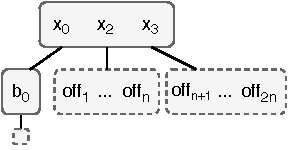
\includegraphics[width=0.3\linewidth]{colt.pdf}
%   \caption{A \COLT for the relation $S$ in
%     Fig.~\ref{fig:clover-query}. Each off$_i$ is an integer
%     representing an offset into the table $S$.}
%   \label{fig:colt}
% \end{figure}

% A \COLT tree need not be balanced, and there can be both hash maps and
% vectors at the same tree level.  Fig.~\ref{fig:colt}
% illustrates a \COLT tree for the instance $S$ of the clover query
% $Q_\clubsuit$.

% %%% \begin{example}\label{ex:colt}
% %%%   Recall the relation $S$ for the clover query $Q_\clubsuit$, 
% %%%   whose \GHTs are shown in Figure~\ref{fig:ght-examples}.
% %%%   Figure~\ref{fig:colt} shows a \COLT for $S$.
% %%% \end{example}


% \begin{figure}
%   \begin{lstlisting}
% struct COLT {
%   relation, schema, vars, 
%   data = Map(HashMap<Tuple, COLT>) | Vec<Vec<u64>> }

% impl GHT for COLT:
%   fn new(relation, schema):
%     COLT { relation, schema, schema[0],
%            data = [ 0, 1, ..., relation.len - 1 ] }

%   fn iter():
%     match self.data:
%       Map(m) => m.keys().iter(),
%       Vec(v) => 
%           if is_suffix(self.vars, relation.schema):
%             v.map(|i| cols = self.relation[self.vars];
%                       cols.map(|c| c[i]) )
%           else: self.force(); self.iter()

%   fn get(key): self.force(); self.get_map.get(key)

%   fn force():
%     match self.data:
%       Map(m) => {} # already forced, do nothing
%       Vec(v) => 
%         map = new()
%         for i in v:
%           cols = self.relation[self.vars]
%           k = cols.map(|col| col[i])
%           if map[k] is None: # make a new, empty COLT
%             map[k] = COLT { relation: self.relation, 
%                             schema: self.schema[1..], 
%                             data: [] }
%           map[k].data.push(i)
%         self.data = Map(map)
% \end{lstlisting}
%   \caption{The \COLT data structure.}
%   \label{fig:colt-impl}
% \end{figure}

% % \ds{I did not understand the rest of this section.  What is needed:
% %   (a) explain how the raw data is stored.  For example, how is a
% %   relation $R(x,y,z)$ stored: row-wise? column-wise? sorted? (b) where
% %   are the indices pointing to?  For example, if I construct the first
% %   level of $R(x,y,z)$, then for each value of $x$ I have a set of
% %   indices: where are these indices pointing to?}
% % \rw{I added an example to explain this.}

% \COLT Implements the \GHT interface in Figure~\ref{fig:ght}, and its
% implementation is shown in Figure~\ref{fig:colt-impl}. As before,
% \COLT stores a reference to the relation it represents, as well as the
% \GHT schema computed from the plan.
% %%% Recall the $i$-th element of the schema contains the variables at
% %%% the $i$-th level of the trie.  For a (sub-)\COLT at level $k$,
% %%% \lstinline|vars| is the same as the $k$-th element of the
% %%% schema. the $0$-th element of the schema.
% Consider a relation with $n$ tuples.  The \COLT tree is initialized
% with a single node consisting of the vector $[0, \ldots, n-1]$,
% i.e. one offset to each tuple.  
% \COLT
% implements the \lstinline|get| and \lstinline|iter| methods lazily.  
% When
% \lstinline|get| is called, we check if the current node is a hash
% map or a vector.  In the first case, we simply perform a lookup in the
% map.  In the second case, we first replace the current vector with a
% hash map, whose children are vectors of offsets.  Notice that this
% requires iterating over the current vector of offsets, accessing the
% tuple in the base table, inserting the key in the hash map, and
% inserting the offset in the corresponding child.  Consider now a call
% to \lstinline|iter|.  If the current node is a hash map, then we
% return an iterator over it.  If it is a vector, then we check if it is
% a suffix of the relation schema: if yes, then we simply iterate over
% that vector (and access the tuples via their offsets), otherwise we
% first materialize the current hash map as explained above, and return
% an iterator over the hash map.

% As a simple but effective optimization, we do not initialize the \COLT
% tree to the single node $[0,1,\ldots,n-1]$, but instead iterate
% directly over the base table, if required.  If no \lstinline|get|
% is performed on this table, then we have completely eliminated the
% cost of building any auxiliary structure on this table.  Thus, the \FJ
% plan can be equivalent to a left-deep plan that avoids building a hash
% table on the left-most relation.  \COLT is also closer to the structure of
% traditional hash tables, which, in some implementations, map a key to
% a vector of pointers to tuples.
% %
% %%% Note that the \COLT for each relation of size $n$ is always initialized to be the 
% %%%   vector $[0, \ldots, n-1]$.
% %%% Since we can only iterate over this vector, 
% %%%   we did not have to materialize it in the first place.
% %%% Instead, we can simply loop over the tuples in the original relation 
% %%%   when \lstinline|iter| is called.
% %%% This means when the \FJ plan is equivalent to a binary plan, 
% %%%   we completely eliminate the cost of trie building for the left relation, 
% %%%   recovering the behavior of binary join.
% %
% %%% \COLT also captures the structure of hash tables more closely than
% %%% \GHTs.  Recall that a hash table maps each key to an entire tuple in
% %%% the relation.  Equivalently, we can also map the key to the row index
% %%% of the tuple.  But that is precisely a \COLT whose first level is
% %%% materialized.

% \begin{example}\label{ex:colt-clover}
% Consider an extension of the clover query $Q_\clubsuit$:
% \begin{align*}
%   Q(x, a, b, c) \cd R(x,a), S(x,b), T(x, c), \underline{U(b)}.
% \end{align*}
%   % 
% %   \begin{lstlisting}[
% %     language=SQL,
% %     showspaces=false,
% %     basicstyle=\ttfamily\small,
% %     commentstyle=\color{gray},
% %     escapeinside={(*}{*)},
% %  ]
% % SELECT * FROM R,S,T,U -- schema: R(x,a),S(x,b),T(x,c),U(b)
% %  WHERE R.x = S.x AND S.x = T.x AND T.x = R.x AND (*\underline{S.b = U.b}*)
% % \end{lstlisting}
% %
% \GJ builds a 2-level hash trie for each of $R$, $S$, and $T$, as well
% as a 1-level hash trie for $U$.  Consider the \FJ plan
% $[[R(x,a),S(x),T(x)],[U(b),S(b)],[T(c)]]$.  \FJ executes the first
% node of the plan by iterating over $R$ directly, without constructing
% any auxiliary structure. For each tuple $(x, a)$ in $R$, it looks up
% $x$ in $S$ and $T$.  Upon the first lookup, \COLT builds the first
% level of the \GHT for $S$ and $T$, i.e. a hash map indexed by the $x$
% values.  Assuming the database instance for $R,S,T$ shown in
% Fig.~\ref{fig:clover-query}, the result of $R.x \cap S.x \cap T.x$ has
% only one value, $x_0$, thus, $\FJ$ executes the second node for only
% one value $x_0$.  Here it needs to intersect $U(b)$ and $S(b)$.
% Assume for the moment that \FJ chooses $U(b)$ to be the cover, on the
% first lookup in $S$, \COLT will expand the second level, arriving at
% Figure~\ref{fig:colt}: notice that all other $b$ values in $S$ will
% never be inserted in the hash table.  More realistically, \FJ follows
% the principle in \GJ and chooses $S(b)$ as cover, because it is the
% smallest: it builds a hash map for $U$, but none for the 2nd level of
% $S$.
% \end{example}

% The example highlights a divergence between \GJ and traditional plans.
% To intersect $R_1.x \cap R_2.x \cap \ldots$, \GJ choose to iterate
% over the smallest relation, which results in the best runtime {\em
%   ignoring} the build time.  A traditional join plan will iterate over
% the largest relation, because then it needs to build hash tables only
% on the smaller relations.  Currently, we follow \GJ, and plan to
% explore alternatives in the future.

% % \ds{Remy please check the example and the discussion}


% % \ds{The example doesn't help.  Once we have identified the single
% %   value $b_0$, we only need to look it up in $U(b)$.  But since we
% %   haven't constructed anything for $U$ yet, this requires a full scan
% %   of $U$.  This is modestly better than scanning $U$ to create a
% %   hash-table, but I don't see how this savings generalizes.  If the
% %   previous joins return the values $b_0, b_1, b_2, \ldots$, then how
% %   can we look them up in $U$ more efficiently than computing a hash
% %   table on $U$?}
% % \rw{Scanning $U$ while probing into the small trie is much faster than 
% % building a hash table for $U$, since the latter needs to allocate memory.
% % But the main point is not about $U$, but rather we avoid building a large 
% % part of the second level of $S$.  }

% \subsection{Vectorized Execution}\label{sec:vectorized-execution}
% The \FJ algorithm as presented in Figure~\ref{fig:fj-algo}
%   suffers from poor temporal locality.
% In the body of the outer loop, 
%   we probe into the same set of relations for each tuple.
% However, these probes are interrupted by the recursive 
%   call at the end, 
%   which is itself a loop interrupted by further recursive calls.

% \begin{figure}
%   \begin{lstlisting}
% @outer for ts in tries[0].iter_batch(batch_size):
%   tup_subtries = [(tuple + t, [ tries[0].get(t) ]) | t $\in$ ts]
%   for trie in tries[1..]:
%     for (tup, subtries) in tup_subtries:
%       subtrie = trie.lookup(tup[trie.vars])
%       if subtrie is None:
%         tup_subtries.remove((tup, subtries))
%       else: subtries.append(subtrie)
%   for (tup, subtries) in tup_subtries:
%     new_tries = all_tries[tries $\mapsto$ subtries]
%     join(new_tries, plan[1:], tup)
% \end{lstlisting}
%   \caption{Vectorized execution for \FJ.}
%   \label{fig:vectorized-execution}
% \end{figure}

% A simple way to improve locality is to perform a batch of probes 
%   before recursing, just like the classic vectorized execution 
%   for binary join.
% Concretely, we replace the \lstinline|iter| method 
%   with a new method \lstinline|iter_batch(batch_size)|
%   which returns up to \lstinline|batch_size| tuples at a time.
% If there are less than \lstinline|batch_size| tuples left, 
%   it returns all the remaining tuples.
% Then we replace the outer loop in Figure~\ref{fig:fj-algo} 
%   with the one in Figure~\ref{fig:vectorized-execution}.
% For each batch of tuples, 
%   we create a vector pairing each tuple to its subtrie in 
%   \lstinline|tries[0]|.
% Then for each trie to be probed,
%   we iterate over the vector and look up each tuple 
%   from the trie.
% If the lookup succeeds, we append the subtrie to the vector of tries paired with the tuple.
% If it fails, we remove the tuple to avoid probing it again.
% Finally, with each tuple and the subtries it pairs with, 
%   we recursively call \lstinline|join|.

% \subsection{Discussion}\label{sec:fj-gj-multijoin}

% \COLT is a lazy data structure, sharing a similar goal with database
% cracking~\cite{DBLP:conf/cidr/IdreosKM07,DBLP:conf/sigmod/IdreosKM07}, where an
% index is constructed incrementally, by performing a little work during each
% lookup. 
% % \rw{Dan, can you check the following?}
% Another connection is to Factorized Databases~\cite{DBLP:journals/sigmod/OlteanuS16} -- we
% intentionally used the term ``factor'' when describing how we optimize \FJ plans to
% suggest this connection. 
% Concretely, we can view the trie data structure as a
% factorized representation of a relation, where keys of the same hash map are
% combined with union, and tuples are formed by taking the product of values at
% different levels. Practically, we can use this factorized representation to 
% compress large outputs, saving time and space during materialization.

% As we discussed at the end of Section~\ref{sec:free-join}, in order
% match the optimality of \GJ, the \FJ algorithm needs to choose
% dynamically the ``cover'', i.e. the relation over which to iterate.  To
% achieve this, we first find {\em all} covers for each node, then make a simple
% change to the \FJ algorithm in Figure~\ref{fig:fj-algo}: we simply
% choose to iterate over the cover whose trie has the fewest keys.  For
% that we insert the following code right before the outer loop in
% Figure~\ref{fig:fj-algo}:
% %
% \begin{lstlisting}
% trie[0] = covers(plan[0]).min_by(|t| t.keys().len)
% trie[1..] = # the rest of the tries
% \end{lstlisting}
% %
% When we use \COLTs, we cannot know the exact number of keys in a vector unless
%   we force it into a hash map. In that case we use the length of the vector as
%   an estimate.

% \begin{example}
%   Consider the triangle query $Q_\triangle$, and the following \FJ plan:
%   $$[[R(x), T(x)], [R(y), S(y)], [S(z), T(z)]]$$  Each subatom is a
%   cover of its own node.  On the outermost loop, we iterate over $R$
%   if it has fewer $x$ values, and otherwise we iterate over $T$.  On
%   the second loop level we make a decision picking between $S$ and a
%   subtrie of $R$, \emph{for each subtrie of $R$}.  Finally, on the
%   innermost loop we pick between the subtries of $S$ and $T$.
% \end{example}

% % \ds{I recommend removing the paragraph below}
% % Another small tweak allows \FJ to further capture other classic
% % multiway joins. Just like how \GJ dynamically choose the relation to iterate
% % over, various classic multiway joins, such as Hash Team~\cite{} and Eddies~\cite{},
% %  also dynamically orders the relations to
% % probe into. We support this by inserting another line right before the 
% % inner loop of Figure~\ref{fig:fj-algo}:
% % %
% % \begin{lstlisting}
% % tries[1..].sort_by(probe_cost)
% % \end{lstlisting}
% % %
% % Here \lstinline|probe_cost| estimates the cost of probing into each trie.
% % The simplest cost function returns the size of the trie;
% % a more advanced one may perform some form of selectivity estimation;
% % and a sophisticated cost model can even receive feedback from previous 
% % iterations of the loop.
\section{Experiments}\label{sec:eval}

% \ds{The section looks good overall.  I made only stylistic changes,
%   mostly in the beginning.  Regarding the Latex layout, I don't
%   onecolumn should be the solution, but instead you should use a
%   figure$*$, then subfigures.  Also, I think you can squeeze in
%   another graph, i.e. arrange them $3 \times 3$.}

We implemented \FJ as a standalone Rust library.  The main entry point
of the library is a function that takes a binary join plan (produced
and optimized by DuckDB), and a set of input relations.  The system
converts the binary plan to a \FJ plan, optimizes it, then runs it
using \COLT and vectorized execution.
%%% The binary plan can be produced by any query optimizer, and we
%%% convert the binary plan into a \FJ plan and further optimize it as
%%% described in Section~\ref{sec:bj-to-fj}.
% In addition to joins, our implementation supports 
%   projection and aggregation, 
%   but relies on an external system for selection.
We compare \FJ against two baselines: our own \GJ implementation in
Rust, and the binary hash join implemented in the state-of-art
in-memory database
DuckDB~\cite{DBLP:conf/cidr/RaasveldtM20,DBLP:conf/vldb/Raasveldt22}.
We evaluate their performance on the popular Join Order Benchmark
(JOB)~\cite{DBLP:journals/pvldb/LeisGMBK015}.
We refer the reader to our SIGMOD paper~\cite{10.1145/3589295}
for additional experiments that include other systems
and benchmark, as well as detailed ablation studies of the optimizations.


% \clearpage
% \onecolumn
\subsection{Setup}

While we had easy access to optimized join plans produced by DuckDB,
we did not find any system that produces optimized \GJ plans,
or can take an optimized plan as input.
%%% 
%%% In addition to using DuckDB as a baseline implementation of binary
%%% join, we use its query optimizer to generate the starting binary plan
%%% that we convert into a \FJ plan.
%%% %
%%% Compared to binary join implementations, 
%%%   there are few systems that implement \GJ, 
%%%   and none of them outputs a machine-readable query plan,
%%%   or can take one as input.
We therefore implement a \GJ baseline ourselves,
by modifying \FJ to fully construct all tries, and removing
vectorization.  We chose as variable order for \GJ the same as for
\FJ.\footnote{\FJ defines only a partial order; we extended it to a
  total order.}

%%% It is essentially \FJ but without the optimizations:
%%%   its execution is not vectorized, and
%%%   instead of using \COLT, it fully constructs every trie ahead of time.
%%% We are not aware of any other algorithm converting a binary plan into a \GJ plan, 
%%%   so we use the same plan for both \FJ and \GJ to ensure a fair comparison.

The JOB benchmark contains 113 acyclic join queries with an average of 8 joins per query.
Each query in the benchmarks only contains base-table filters,
natural joins, and a simple group-by at the end,
and no null values.
The queries works over real-world data from the IMDB dataset.
We exclude 5 queries that return empty results,
since such empty queries are known to introduce reproducibility issues\footnote{
  See GitHub issue: https://github.com/gregrahn/join-order-benchmark/issues/11
}.

We ran all our experiments on a MacBook Air laptop with Apple M1 chip and 16GB memory.
All systems are configured to run single-threaded in main memory,
and we leave all of DuckDB's configurations to be the default.
All systems are given the same binary plan optimzed by DuckDB.
Since we are only interested in the performance of the join algorithm,
we exclude the time spent in selection and aggregation
when reporting performance.
This excluded time takes up on average less than 1\% of the total execution time.

\begin{figure}
  \centering
  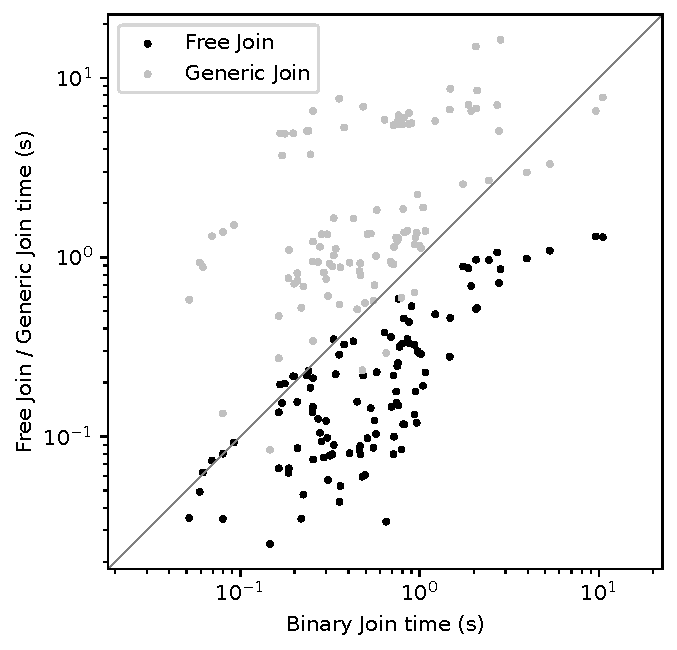
\includegraphics[width=.9\linewidth]{imdb.pdf}
  \captionof{figure}{Run time comparison on JOB.
    Each black dot compares the run time of a query on \FJ and binary join,
    and a black dot below the diagonal means \FJ is faster.
    The gray dots compare \GJ and binary join similarly.
  }
  \label{fig:eval:imdb}
\end{figure}%

\begin{figure}
  \centering
  \begin{tabular}{c}
    \begin{lstlisting}[numbers=none]
111101
JOIN
 |  \________9775
1919495      company_name(cid)
JOIN
 |  \________1
8123586      company_type(ctid)
JOIN
 |  \________1
24740873     info_type1(iid1)
JOIN
 |  \________1
148621556    info_type2(iid2)
JOIN
 |  \________1
177388547    kind_type(kid)
JOIN
 |  \________2609129
20885030     movie_companies(mid, cid, ctid)
JOIN
 |  \________1380035
 |           JOIN
 |            |  \_____1380035
 |           2528312   movie_info_idx(mid, iid1)
 |           title(mid, kid)
14835720    
movie_info(mid, iid2) 
\end{lstlisting}
  \end{tabular}
  \caption{Query plan produced by DuckDB for JOB Q13a.
    We show the join attributes next to each input relation,
    and label each relation with its size as well as
    each join with its (actual) cardinality.  }
  \label{fig:eval:imdb:plan}
\end{figure}


% \end{lstlisting}
% \end{figure*}

% \begin{figure*}
%   \centering
%   \begin{minipage}[t]{.45\textwidth}
%     \centering
%     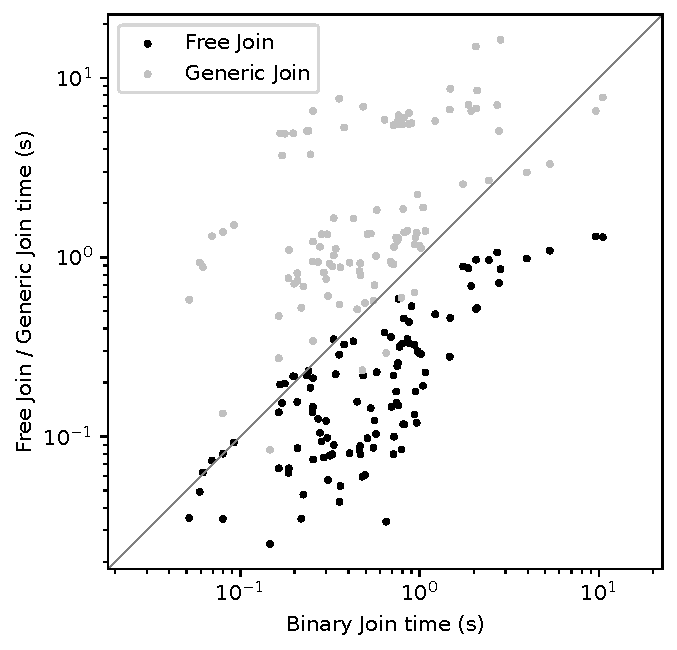
\includegraphics[width=\linewidth]{imdb.pdf}
%     \captionof{figure}{Run time comparison on JOB.
%       Each black dot compares the run time of a query on \FJ and binary join,
%       and a black dot below the diagonal means \FJ is faster.
%       The gray dots compare \GJ and binary join similarly.
%     }
%     \label{fig:eval:imdb}
%   \end{minipage}%
%   \hspace{1em}
%   \begin{minipage}[t]{.45\textwidth}
%     \centering
%     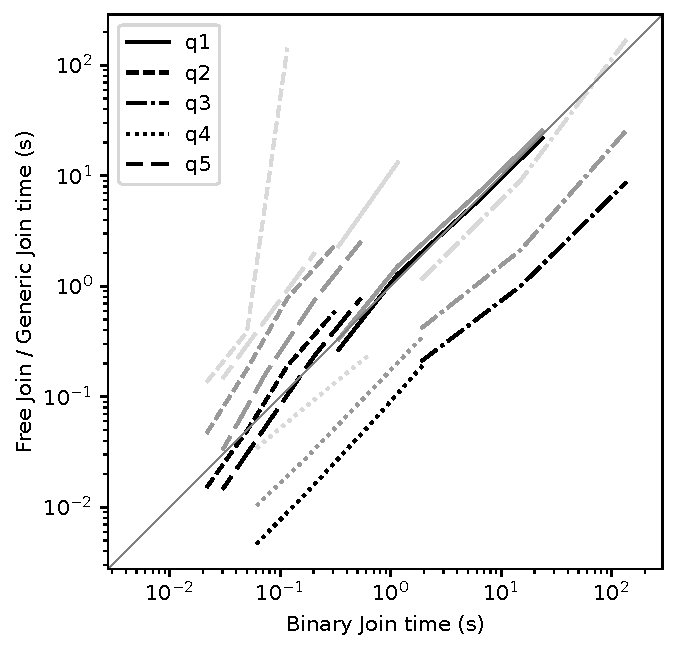
\includegraphics[width=\linewidth]{lsqb-slow.pdf}
%     % \captionof{figure}{\FJ and \GJ v.s.\ binary join on LSQB queries.
%     % Each line is a query running on increasing scaling factors (0.1-3).
%     % Grey lines are for \GJ, and black lines are for \FJ.
%     % }
%     \captionof{figure}{Run time comparison on LSQB.
%       Each line is a query running on increasing scaling factors (0.1, 0.3, 1, 3).
%       The black lines compare \FJ with binary join,
%       the gray lines compare our \GJ baseline with binary join,
%       and the light gray lines compare K\`uzu with binary join.
%     }
%     % Grey lines are for \GJ, and black lines are for \FJ.
%     % }
%     \label{fig:eval:lsqb}
%   \end{minipage}
% \end{figure*}


\subsection{Run time comparison}\label{sec:run-time-comparison}

Figure~\ref{fig:eval:imdb} compares the run time of \FJ and \GJ against binary join on JOB queries.
We see that almost all data points for \FJ are below the diagonal,
indicating that \FJ is faster than binary join.
On the other hand, the data points for \GJ are largely above the diagonal,
indicating that \GJ is slower than both binary join and \FJ.
On average (geometric mean), \FJ is \imdbavgfjbj faster than binary join
and \imdbavgfjgj faster than \GJ.
The maximum speedups of \FJ against binary join and \GJ
are \imdbmaxfjbj and \imdbmaxfjgj, respectively,
while the minimum speedups are \imdbminfjbj (\imdbmaxbjfj slowdown) and \imdbminfjgj.

We zoom in onto a few interesting queries for a deeper look.
The slowest query under DuckDB is Q13a, taking over 10 seconds to finish.
\GJ runs slightly faster, taking 7 seconds,
whereas \FJ takes just over 1 second.
The query plan for this query,
as shown in Figure~\ref{fig:eval:imdb:plan},
reveals the bottleneck for binary join:
the first 3 binary joins are over 4 very large tables,
and two of the joins are many-to-many joins, exploding the
intermediate result to contain over 100 million tuples.
However, all 3 joins are on the same attribute (\lstinline|mid|);
in other words they are quite  similar to our clover query $Q_\clubsuit$.
As a result, \GJ and \FJ simply intersects the relations
on that join attribute,
expanding the remaining attributes only after
other more selective joins.
% This data point appears to confirm a folklore that claims
% \WCOJ algorithms are more resistant to poor query plans.
% After all, binary join could have been faster, had the query plan
% ordered the more selective joins first.
% We expand on this point with more experiments evaluating
% each algorithm's robustness against poor plans in Section~\ref{sec:robustness}.

On a few queries \FJ runs slightly slower than binary join,
as shown by the data points over the diagonal.
The binary plans for these queries are all bushy,
and each query materializes a large intermediate relation.
We have not spent much effort optimizing for materialization,
and we implement a simple strategy: for each intermediate
that we need to materialize, we store the tuples containing
all base-table attributes in a simple vector.
Future work may explore more efficient materialization strategies,
for example only materializing attributes that
are needed by future joins.

% Figure~\ref{fig:eval:lsqb} compares the performance of \FJ and \GJ against binary join on LSQB queries.
% Each line corresponds to one query running on scaling factors 0.1, 0.3, 1, and 3.
% The black lines are for \FJ, gray lines for our own \GJ baseline, and light gray lines for K\`uzu.
% K\`uzu errors when loading data for SF3;
% it did not finish after 10 minutes for q1 SF 1.
% DuckDB also took over 10 minutes running q3 SF 3.
% These instances do not show up in the figure.
% We can see K\`uzu takes consistently longer than our \GJ implementation
% on all queries across scaling factors.
% This shows that our \GJ implementation is a reasonable baseline to compare against.
% On cyclic queries, \FJ is up to 15.45x (q3) faster than binary join,
% and up to 4.08x (q2) faster than \GJ.
% On acyclic queries \FJ is up to 13.07x (q4) and 3.25x (q5) faster than binary join and \GJ, respectively.
% On q3 and q4 both \FJ and \GJ consistently outperform binary join on all scaling factors.
% q3 contains many cycles, whereas q4 is a star query, so the superior performance of \FJ and \GJ is expected.
% % q1, however, is a chain query, where \WCOJ algorithms are expected to be inefficient.
% % A deeper look reveals q1 to have an output much larger than its inputs, 
% %   but uses a \lstinline|COUNT(*)| at the top.
% % An unintended benefit of \GJ and \FJ is that any attributes that 
% %   do not participate in a join are not expanded, 
% %   so the output result is naturally stored in a \emph{factorized} form.
% % We compute the \lstinline|COUNT| aggregate directly on the factorized output, 
% %   which is much faster than expanding and counting.
% Surprisingly, despite q2 being a cyclic query,
% \FJ is only slightly faster on smaller inputs
% and is even slightly slower on larger inputs.
% This is the opposite of the common believe that \WCOJ algorithms
% should be faster on cyclic queries.
% The query plan reveals that there are no skewed joins,
% and so binary join suffers no penalty.
% Our experience shows that, in practice,
% the superiority of \WCOJ algorithms like \FJ and \GJ
% is not solely determined by the cyclicity of the query;
% the presence of skew in the data is another important factor.

% \begin{figure}
%   \centering
%   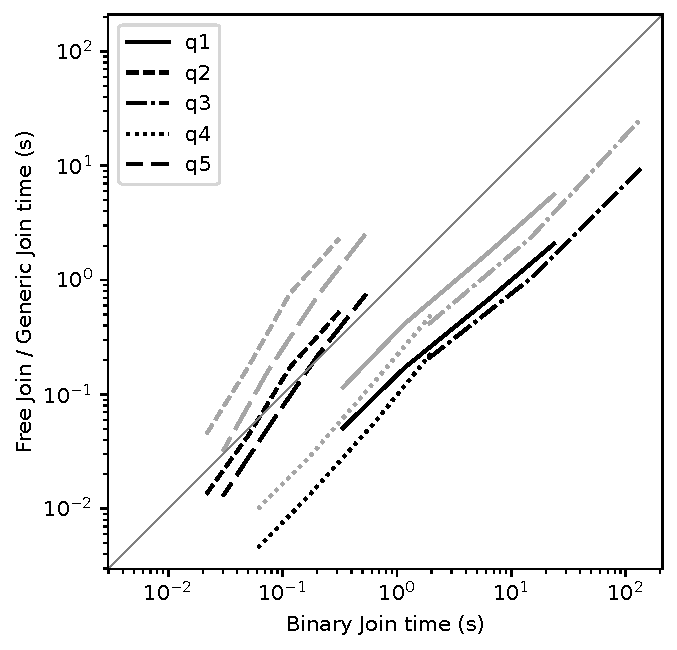
\includegraphics[width=.45\linewidth]{lsqb.pdf}
%   \caption{Run time comparison on LSQB w/ factorization.}
%   \label{fig:eval:lsqb-factor}
% \end{figure}

% Unlike the JOB queries, in LSQB the output size (before aggregation)
% is much larger than the input size.
% This leads to a large amount of time spent in constructing the output,
% which involves random accesses to retrieve the data values for each tuple.
% We therefore implemented the optimization in Section~\ref{sec:fj-gj-multijoin}
% to factorize the output.
% This made q1 significant faster, as shown in Figure~\ref{fig:eval:lsqb-factor},
% while other queries are not affected.

% \begin{figure*}
%   \centering
%   \begin{minipage}{.45\textwidth}
%     \centering
%     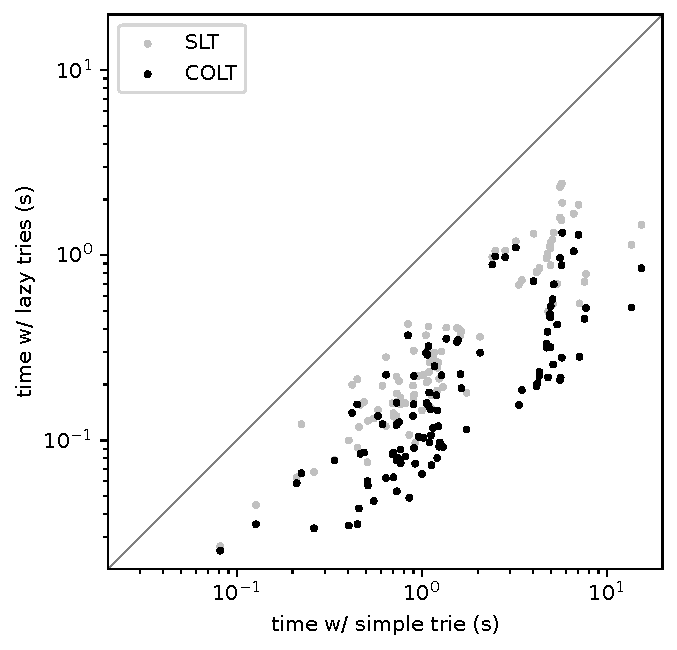
\includegraphics[width=\linewidth]{colt-ab.pdf}
%     \captionof{figure}{Impact of \COLT.}
%     \label{fig:eval:colt-ab}
%   \end{minipage}%
%   \hspace{1em}
%   \begin{minipage}{.45\textwidth}
%     \centering
%     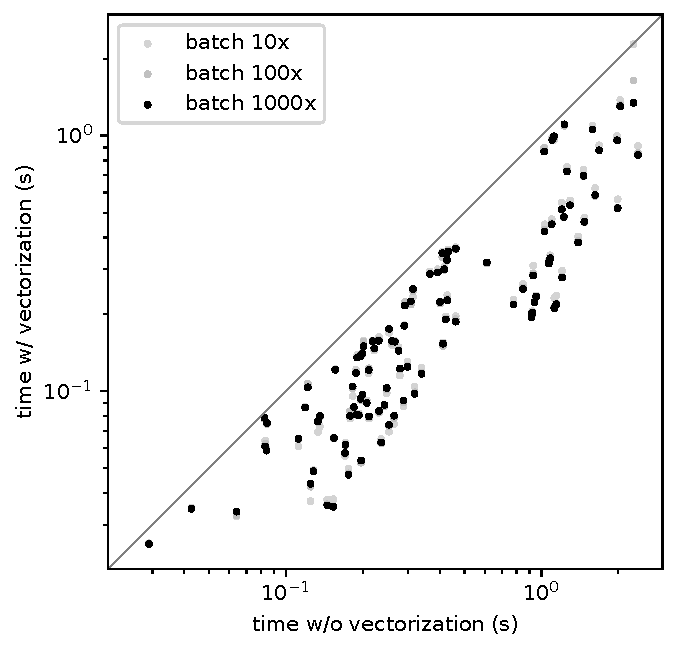
\includegraphics[width=\linewidth]{vec-ab.pdf}
%     \captionof{figure}{Impact of vectorization.}
%     \label{fig:eval:vec-ab}
%   \end{minipage}
% \end{figure*}
% % \subsection{Impact of \COLT and Vectorization}
% % % \ds{Try to choose section titles that are related to the question
% % %   that the section addresses}
% % The three key ingredients that make \FJ efficient
% % are \begin{enumerate*}
% %   \item our algorithm to optimize the \FJ plan by factoring,
% %   \item the \COLT data structure, and
% %   \item the vectorized execution algorithm.
% % \end{enumerate*}
% % We conduct an ablation study to evaluate the performance impact of these components.
% % But if we do not optimize the \FJ plan converted from a binary plan
% % and execute it as-is, \FJ would behave identically to binary join.
% % Since we have already compared \FJ with binary join in Section~\ref{sec:run-time-comparison},
% % we do not repeat it here.
% % Therefore, our ablation study includes two sets of experiments,
% % evaluating the impact of \COLT and vectorization respectively.



% Figure~\ref{fig:eval:colt-ab} compares the run time of \FJ using different trie data structures.
% The baseline fully expands each trie ahead of time, and we call this \emph{simple trie}.
% Another data structure, \emph{simple lazy trie} (SLT), expands the first level of each trie
% ahead of time, while expanding the inner levels lazily.
% This is the same strategy as proposed by Freitag et.al.~\cite{DBLP:journals/pvldb/FreitagBSKN20}.
% Finally, \COLT is our column-oriented lazy trie.
% In all three cases, we use the default vectorization batch size 1000.
% The experiments show the average (geometric mean) speedup of \COLT
% is 1.91x and 8.47x, over SLT and simple trie respectively,
% and the maximum speedup over them is 11.01x and 26.29x, respectively.


% Figure~\ref{fig:eval:vec-ab} compares the run time of \FJ using different vectorization batch sizes.
% The baseline uses no vectorization, i.e., we set the batch size to 1.
% Then we adjust the batch size among 10, 100, and 1000.
% The data does not show significant performance differences among
% the different batch sizes --
% it appears \emph{any amount of vectorization is better than none}.
% For short-running queries, a smaller batch size perform slightly better,
% and for longer running queries a larger batch size wins.
% We conjecture this is due to a smaller batch having less overhead,
% leading to lower latency,
% while a larger batch size speeds up large joins better,
% leading to better throughput.
% Overall, using the default batch size 1000
% leads to an average (geometric mean) speedup of 2.12x,
% and a maximum speedup of 5.33x over non-vectorized \FJ.

% \begin{figure*}
%   \begin{minipage}{.45\textwidth}
%     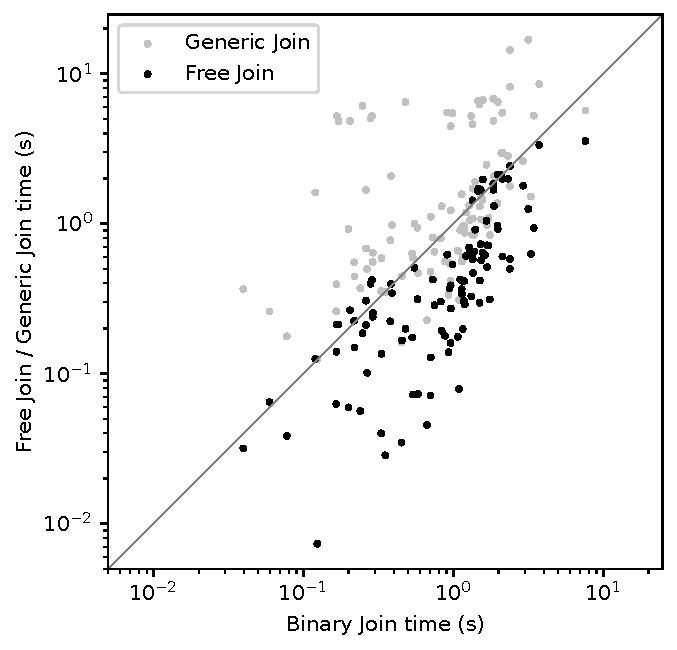
\includegraphics[width=\linewidth]{robust.pdf}
%   \end{minipage}
%   \hspace{1em}
%   \begin{minipage}{.45\textwidth}
%     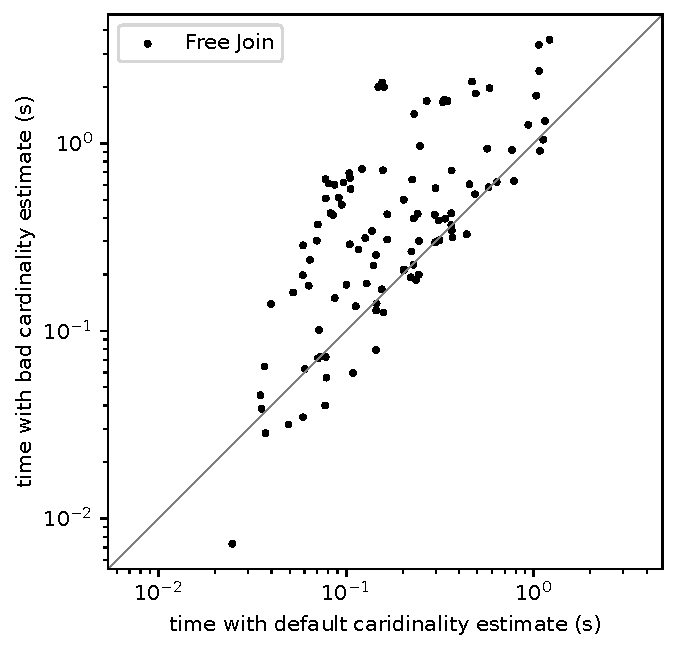
\includegraphics[width=\linewidth]{robust_fj.pdf}
%   \end{minipage}
%   \begin{minipage}{.45\textwidth}
%     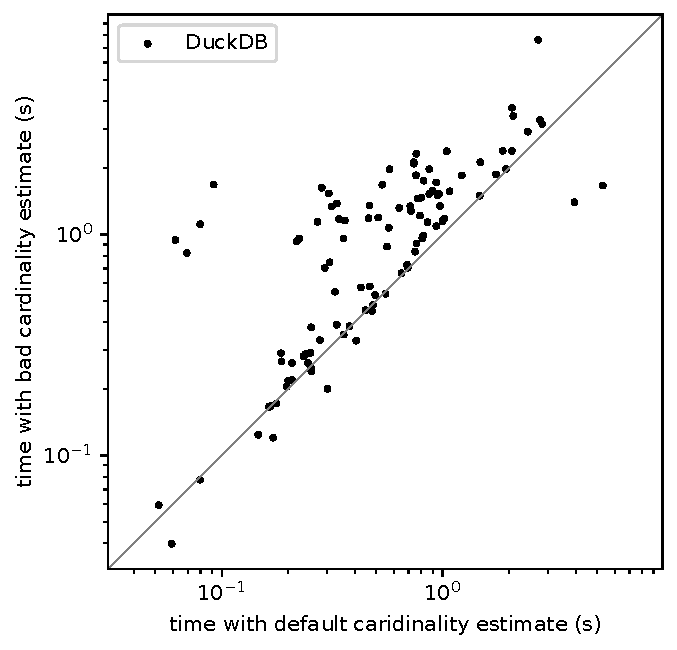
\includegraphics[width=\linewidth]{robust_bj.pdf}
%   \end{minipage}
%   \hspace{1em}
%   \begin{minipage}{.45\textwidth}
%     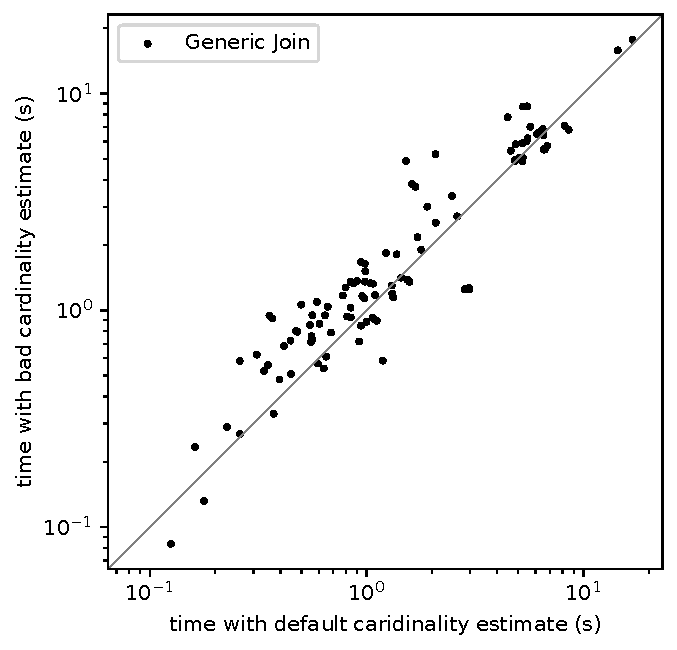
\includegraphics[width=\linewidth]{robust_gj.pdf}
%   \end{minipage}
%   \caption{Run time of join algorithms with good and bad cardinality estimates.
%     The first plot compares the run time of \FJ, \GJ and binary join
%     on JOB with bad cardinality estimates.
%     The remaining three plots compare the run time of each algorithm
%     with good and bad cardinality estimates on JOB.
%   }
%   \label{fig:sensitivity}
% \end{figure*}

% \subsection{Robustness Against Poor Plans}\label{sec:robustness}

% Our last set of experiments compares \FJ, \GJ and binary join
% on their sensitivity to the quality of the query plan.
% Many believe \WCOJ algorithms suffer less from poor query planning,
% due to its asymptotic guarantees.
% Our experience with Q13 from Section~\ref{sec:run-time-comparison}
% also seems to confirm this intuition.
% However, our experimental results tell a different story.
% As the first plot in Figure~\ref{fig:sensitivity} shows,
% the relative performance of the three algorithms stays
% the same with good and bad plans, with \FJ being the fastest,
% \GJ the slowest, and binary join in the middle.
% However, as shown in Figure~\ref{fig:sensitivity},
% \FJ seems to slow down as much as binary join
% when the plan is bad (there are many points far above the diagonal).
% It turns out with a poor cardinality estimate,
% DuckDB routinely outputs bushy plans that materialize large results.
% We have noted in Section~\ref{sec:run-time-comparison} that
% our materialization strategy is simplistic,
% so with larger intermediates it leads to more severe slowdown.
% In comparison, \GJ slows down less (the data points are close to the diagonal).
% However, it was the slowest to begin with,
% and since overheads like trie building dominates \GJ's run time,
% a bad plan does not make it much slower.
% Overall, we believe \FJ can be more robust to bad plans with
% faster materialization.

\section{Limitations and Future Work}\label{sec:discussion}

With \FJ we have made a first step to bring together 
the worlds of binary join and \WCOJ algorithms.
There are three obvious limitations that require future work.  Our
current system is main memory only.  If the data were to reside on
disk, then \COLT could be quite inefficient, because it requires
repeated, random accesses to the data.  Another limitation is that the
optimization of a \FJ plan is split into two phases: a
traditional cost-based optimization (currently done by DuckDB),
followed by a heuristic-based optimization of the \FJ plan
(factorization).  This has the advantage of reusing an existing
cost-based optimizer, but the disadvantage is that an integrated
optimizer may be able to find better plans.  Third, our current
optimizer does not make use of existing indices.  It is known that the
optimization problem for join plans becomes harder in the presence of
foreign key indices~\cite{DBLP:journals/pvldb/LeisGMBK015}, and we
expect the same to hold for \FJ plans.  All these limitations require
future work.  As we have designed \FJ to closely capture binary join
while also generalizing it, we hope the solutions to these problems
can also be smoothly transferred from binary join to \FJ.

Finally, we have made several observations during this project, some
of them quite surprising (to us), which we believe deserve a future
study.  We observed that a major bottleneck is the materialization of
intermediate results in bushy plans; an improved materialization
algorithm may speed up \FJ on bushy plans.  One promising idea is to
be more aggressively lazy and keep \COLTs unexpanded during
materialization, which essentially leads to a factorized
representation of the intermediates.  We also observed that, contrary
to common belief, a cyclic query does not necessarily mean \WCOJ
algorithms are faster, and an acyclic query does not mean they are
slow.  A natural question is thus ``when exactly are \WCOJ algorithms
faster than binary join?''  Answering this question will also help us
design a better optimizer for \FJ.  The optimizer can output a plan
closer to \WCOJ when it expects major speedups.  We note that the
query optimizer by~\cite{DBLP:journals/pvldb/FreitagBSKN20} switches
between \GJ and binary join depending on the estimated cardinality.
In contrast, an optimizer for \FJ should smoothly transform a \FJ plan
to fully explore the design space between the two extremes of binary
join and \GJ.  Finally, we realized that, rather surprisingly, \GJ and
traditional joins diverge in their choice of the inner table (called
the cover in our paper): \GJ requires that to be the smallest
(otherwise it is not optimal), while a traditional plan will chose it
to be the largest (to save the cost of computing its hash table).
Future work is required for a better informed decision for the choice
of the inner relation.


%%% Yet, we have been working with the most basic forms 
%%%   of the algorithms, where the data fits into main memory, 
%%%   the algorithms use a single thread. 
%%% Some natural questions to answer next include: 
%%% \begin{itemize}
%%%     \item What data structures can make \FJ efficient on disk?
%%%     \item How can we take advantage of multi-cores to scale up \FJ? And what about distributed \FJ?
%%%     \item How can \FJ make use of indices?
%%% \end{itemize}
%%% These problems have all been well-studied in the context of binary join. 
%%% As we have designed \FJ to closely capture binary join while also generalizing it, 
%%%   we hope the solutions to these problems can also be smoothly transferred 
%%%   from binary join to \FJ.
%%% 
%%% We designed \FJ to take as input an already optimized binary plan, 
%%%   so that it is easy to integrate \FJ into an existing system.
%%% Nevertheless, we expect an optimizer designed for \FJ will find 
%%%   better plans than a traditional optimizer designed for binary join.
%%% Designing optimization algorithms for \FJ can therefore be an 
%%%   important research direction.
%%% 
%%% Throughout the experiments, we have observed one major bottleneck to be the
%%%   materialization of intermediate results. A better materialization algorithm
%%%   than ours may further speed up \FJ on bushy plans. One promising idea is to be
%%%   more aggressively lazy and keep \COLTs unexpanded during materialization, 
%%%   which essentially leads to a factorized representation of the intermediates.
%%% 
%%% Through experiments, we have observed that a cyclic query does not necessarily 
%%% mean \WCOJ algorithms are faster, and an acyclic query does not mean they are slow.
%%% A natural question is thus ``when exactly are \WCOJ algorithms faster than binary join?''
%%% Answering this question will also help us design a better optimizer for \FJ.
%%% The optimizer can output a plan closer to \WCOJ when it expects major speedups. 
%%% We note that the query optimizer by~\cite{DBLP:journals/pvldb/FreitagBSKN20} 
%%%   switches between \GJ and binary join depending on the estimated cardinality.
%%% In contrast, an optimizer for \FJ should smoothly transform a \FJ plan 
%%%   to fully explore the design space between the two extremes of binary join and \GJ.
% \section{Related Work}\label{sec:related}
% \section{Conclusion}\label{sec:conclusion}

% \clearpage

\begin{acks}
  We thank Winston Bullen for his important contributions to
  experimental infrastructures of this project.
  This work is supported by
  NSF-BSF 2109922, NSF IIS 1954222, and NSF IIS 1907997.
\end{acks}

% \balance

\bibliographystyle{ACM-Reference-Format}
\bibliography{references}

% \clearpage

% \section{\GJ v.s. Binary Join}

% \ds{This detailed description does not belong to the introduction;
%   here it suffices to say that \FJ outperforms traditional plans even
%   on cyclic queries, namely star queries.}  
% \ds{In fact your example
%   shows that \GJ is asympotitically faster than traditional plans even
%   on acyclic queries: explain $O(n)$ v.s. $O(n^2)$.  The reason is
%   that acylic queries do not implement Yannakakis faithfully.}
For an intuition of why \GJ may be faster than binary join, 
  consider the following query:
  \begin{lstlisting}[
    language=SQL,
    showspaces=false,
    basicstyle=\ttfamily\small,
    numbers=left,
    numberstyle=\tiny,
    commentstyle=\color{gray}
 ]
SELECT * FROM R, S, T -- schema: R(x,a), S(x,b), T(x,c)
 WHERE R.x = S.x AND S.x = T.x AND T.x = R.x
\end{lstlisting}
Note that this query is \emph{acyclic}.
A database instance for \texttt{R}, \texttt{S}, and \texttt{T} 
  is shown in Figure~\ref{fig:sand-dollar}.
We will refer to this query and database instance as the \emph{sand dollar query}.
There are only 4 values for the attribute $x$ in the database:
  $\set{x_0, x_1, x_2, x_3}$.
There are $2n+1$ values for each of $a$, $b$ and $c$:
  $\set{a_0, a_1^l, \ldots, a_n^l, a_1^r, \ldots, a_n^r}$, 
  and similar for $b$ and $c$. 
The relations $R$, $S$ and $T$ are as follows:
%
\begin{align*}
  R & = \set{(x_0, a_0)} \cup \bigcup_{i \in [1 \ldots n]} \set{(x_1, a_i^l), (x_2, a_i^r)} \\
  S & = \set{(x_0, b_0)} \cup \bigcup_{i \in [1 \ldots n]} \set{(x_2, b_i^l), (x_3, b_i^r)} \\
  T & = \set{(x_0, c_0)} \cup \bigcup_{i \in [1 \ldots n]} \set{(x_3, c_i^l), (x_1, c_i^r)} 
\end{align*}
%
It should be clear that the only output tuple is $(x_0, a_0, b_0, c_0)$.
To answer this query,
  any binary join plan must first join two of the relations,
  producing $n^2 + 1$ tuples.
For example, joining $R$ with $S$ produces the tuple $(x_0, a_0, b_0)$
  as well as the tuples $\setof{(x_2, a_i^r, b_j^l)}{i, j \in [1 \ldots n]}$.
$n^2$ of these tuples are only to be discarded by the join 
  with the third relation, leaving only one output tuple.
\GJ, on the other hand, joins all three relations at the same time.
The algorithm proceeds as follows:
\begin{enumerate}
  \item Build a hash table for each relation with \texttt{x} as the key.
  \item Take the intersection of the keys of the three hash tables.
  \item For each key in the intersection (there is only one in this example),
  retrieve the corresponding tuples from the hash tables and output them.
\end{enumerate}
Each step in this process takes time linear in the size of the relations,
  in contrast to the quadratic time of the first binary join.
In other words, \GJ is asymptotically faster than \emph{any}
  binary join plan for this acyclic query.
In fact, we will prove that 
\textbf{for any binary plan that runs in time $T(I)$ 
  on a database instance $I$,
  there exists a \GJ plan that runs in time $O(T(I))$}.

\begin{figure}
  \centering
  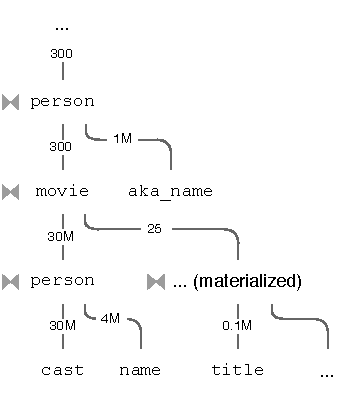
\includegraphics[width=0.7\linewidth]{q56-plan.pdf}
  \caption{
    Fragment of query plan produced by DuckDB.
    The number after each operation counts the output tuples.
  }
  \label{fig:q56-plan}
\end{figure}

Despite the guarantees on asymptotic complexity,
  Mhedhbi and Salihoglu~\cite{} 
  and Freitag et.al.~\cite{} 
  have 
  % \ds{Who has observed that?}
 observed that \GJ can be slow in practice.
Its inefficiency can be demonstrated by the following query fragment\footnote{Simplified for clarity.}
  from the Join Order Benchmark~\cite{DBLP:journals/pvldb/LeisGMBK015}:
%
 \begin{lstlisting}[
   language=SQL,
   showspaces=false,
   basicstyle=\ttfamily\small,
   numbers=left,
   numberstyle=\tiny,
   commentstyle=\color{gray},
   deletekeywords={CAST}
]
SELECT ...
  FROM cast, name, title, aka_name, ... 
 WHERE cast.person = name.person
   AND cast.movie = title.movie
   AND cast.person = aka_name.person
   AND ...
\end{lstlisting}
%
A fragment of the query plan (using binary hash joins) produced by DuckDB 
  is shown in Figure~\ref{fig:q56-plan}.
The first notable detail is the large size of the \texttt{cast} relation.
Since \texttt{cast} is on the left, 
  the binary join simply iterates over each tuple in the relation.
In contrast, \GJ would build a hash table for \texttt{cast},
  which is very expensive.
Here we make a simple yet powerful observation:
  \GJ can simply iterate over certain relations
  instead of building hash tables for them.
In other words, \textbf{we only need to build a hash table 
  for a relation before we probe into it}.
This avoids the cost of building large hash tables, 
  which in our experiments can take much longer 
  than the run time of the entire query.
This example demonstrates the general principle 
  to build hash \emph{lazily}, 
  which is the central idea behind our \COLT data structure.

Another source of inefficiency lies in the main loop of \GJ. 
Looking back at the join plan,
  we see that the first and third joins are not selective,
  while the second join is very selective.
Following this plan, the first two binary joins require
  30 million lookups each, 
  and the third join requires 300 lookups.
In total this sums to a just over 60 million lookups.
\GJ, on the other hand, joins all three relations on \texttt{person}
  at the same time, before the selective join on \texttt{movie}.
This means the join on \texttt{person} incurs 30 million lookups
  each on \texttt{name} and \texttt{aka\_name},
  and the join on \texttt{movie} incurs yet another 30 million lookups.
In total, \GJ performs 90 million lookups.

The root cause of \GJ's inefficiency is that it insists on 
  joining \emph{all} relations involving the same variable at the same time.
Our remedy is to simply relax this requirement,
  delaying certain relations to be joined later.
We call this optimization \textbf{variable splitting}.
In this example, we split the three-way join on \texttt{person}
  into a join between \texttt{cast} and \texttt{name},
  and delay the join on \texttt{aka} 
  until after joining on \texttt{movie}.
By doing so, we recover exactly the original binary plan.

There is another way to improve the performance of \GJ.
Instead of splitting the join on \texttt{person}, 
  we \emph{merge} the joins on \texttt{movie} and \texttt{person}.
Although the original \GJ algorithm can only join on one variable at a time,
  since we iterate over each tuple in \texttt{cast},
  we can join on \texttt{movie} and \texttt{person} at the same time.
In particular, while iterating over \texttt{cast} we may 
  dynamically decide which one of \texttt{name}, \texttt{aka\_name}, 
  and \texttt{title} to probe first.
In this example, it turns out the materialized intermediate
  only contains 25 tuples. 
\GJ can take this runtime information into account
  and prioritize probing the materialized intermediate.
We call this optimization \textbf{variable merging}
  which captures and generalizes classic multiway join algorithms
  like Hash Teams~\cite{} and Eddies~\cite{}.

Variable splitting and merging chart a design space of join algorithms
  that covers both binary join and \GJ, 
  as well as traditional multiway joins.
We illustrate this design space in Figure~\ref{fig:free-join}.
Each point in the design space can be derived by specifying 
  how many variables to join on, 
  as well as how many relations involving those variables to join on.
\textbf{
Being able to join on any number of variables and relations
  frees us from the constraints of existing algorithms.
}
Thereby we unify existing algorithms into a new, 
  general framework called \FJ.

% Through the lens of \FJ, we shall see that binary join and \GJ 
%   are not so different after all.
% In fact, we will show that many of the key techniques
%   that are considered staples of traditional join algorithms 
%   can also be applied to \FJ in a straightforward way.
% Specifically, we propose:
% %
% \begin{itemize}
%   \item \COLT (for \emph{Column-Oriented Lazy Trie}), a column-oriented trie data structure for \FJ
%   \item A vectorized execution algorithm for \FJ 
%   \item An algorithm to convert any binary join plan to a \FJ plan 
%     that runs as fast or faster
% \end{itemize}
% %
% We hope practitioners will find the final point particularly appealing: 
%   it allows them to reuse the existing query optimizer
%   and implement \FJ as a drop-in replacement for binary join.

% In summary, we make the following contributions in this paper:
% \begin{enumerate}
%   \item \FJ, a framework unifying existing join algorithms
%   \item Optimizations to split and merge variables that 
%     improve the performance of \FJ beyond existing algorithms
%   \item Techniques to adapt column-oriented layout, vectorization and query optimization
%     to further speed up \FJ
%   \item A proof that the run time of \GJ is asymptotically bounded by that of binary join
%     on any query and database
%   \item Experiments evaluating the algorithms and optimizations
% \end{enumerate}

\section{Scratch}
\begin{itemize}
  \item A figure showing join plans for binary join, \GJ, and \FJ. 
  \item Index join example.
  \item Architecture diagram.
  \item Column-wise layout.
  \item Benchmarks.
  \item TACO?
\end{itemize}


\subsection{Analysis of Asymptotic Run Time}
\begin{definition}[Left-deep Linear Plan]
  A left-deep linear plan is a sequence of relations. 
  The first relation is called the ``left'' relation.
  Every relation in the sequence joins with all previous
    relations on all common variables.
\end{definition}

\begin{definition}[Step-wise Plan]
  Given a left-deep linear plan, 
    we derive its step-wise plan by expanding
    each join involving more than one variable.
  For each join involving variables $x_1, \ldots, x_n$,
    we replace it with $n-1$ left-semijoins,
    each one on $x_1, \ldots, x_i$ for $i = 1, \ldots, n$,
    followed by the original join.
\end{definition}

\begin{lemma}
  Given a left-deep linear plan running in time $T(I)$
    where $I$ is a database instance,
    its step-wise plan runs in time $O(T(I))$.
\end{lemma}
\begin{proof}
  Each join operation in the left-deep linear plan is replaced
    by a constant number of semijoins plus one natural join
    in the step-wise plan.
  Each semijoin runs in time linear in the run time of the original join,
    and the run time of the final natural join in the step-wise plan
    is also bounded by the run time of the original join.
  Therefore, the total run time of the step-wise plan is linear
    in the run time of the left-deep linear plan.
\end{proof}

\begin{theorem}
  Fix a database $I$. 
  For any binary join plan that runs in time $T(I)$,
   there exists a generic join plan that runs in time $O(T(I))$.
\end{theorem}
\begin{proof}
  We first generate a variable ordering from the binary join plan.
  Given a left-deep linear plan, 
    we generate a variable ordering by traversing the plan bottom-up,
    adding each new variable to the ordering if it has not been added yet.
  If a binary join involves more than 1 variable,
    we visit them in the order they appear in the join.

  Expand the binary plan into a step-wise plan.
  We now prove that \GJ with the variable ordering
    specified above runs in time linear in the run time of the step-wise plan,
    which is linear in the run time of the binary plan.

  Now consider for a given $i$, 
    the $i$-th \GJ loop together with the $i$-th step-wise join.
  Let $l_i$ be the number of iterations of the $i$-th \GJ loop,
    and $t_i$ be the number of tuples arriving at the $i$-th binary join.
  Let $x_1, \ldots, x_{i-1}$ be the first $i-1$ variables in the ordering.
  Then we have: 
%
\begin{align}
    & = t_i
\end{align}
%
  Here we use a few ad-hoc notations to reduce clutter:
  \begin{itemize}
    \item $(x_1 : v_1, x_2 : v_2, \ldots)$ is a tuple where variable $x_a$ has value $v_a$.
    \item $R_j(x_a, x_b, \ldots)$ means some variables $x_a, x_b$ from the tuple appears in the relation $R_j$.
    \item $(v_a, v_b) \in R_j$ means $R_j$ contains a tuple where $x_a = v_a$ and $x_b = v_b$.
  \end{itemize}
  In other words, the set in Equation~\ref{eq:gj-vs-bj:gj} contains only tuples that appear in the join of \emph{all}
    relations that contain variables $x_1, \ldots, x_{i-1}$,
    whereas the set in Equation~\ref{eq:gj-vs-bj:bj} contains tuples that appear in the join of the first $i$ relations
    in the step-wise plan.
\end{proof}

% R(x, y), S(y, z), T(x, z)
\begin{lstlisting}[mathescape=true]
  X = R.x $\cap$ T.x
  for x in X
    Y = R[x].y $\cap$ S.y
    for y in Y
      Z = S[y].z $\cap$ T[x].z
      for z in Z
        yield (x, y, z)
\end{lstlisting}


\subsection{Analysis of absolute run time}
Before we formally analyze the run time of \FJ,
  let us gain some intuition of why \FJ can run faster than binary join.
\begin{example}
  Consider again the ``sand dollar'' query: 
%
  $$Q(x, a, b, c) \cd R(x, a), S(x, b), T(x, c).$$
%
  The plans are nearly identical, 
   except that the free join plan hoists the lookup on $T$ out of the second loop.
  This means that the free join plan makes fewer lookups on $T$.
  Moreover, the middle loop over $b$ in $S$ is also invoked fewer times, 
   since the lookup on $T$ may fail and continue to the next iteration of the outer loop.
\end{example}

With this intuition, we can now prove the absolute run time of \FJ
  is bounded by that of the corresponding binary join plan.

\begin{theorem}
  Fix a database $I$. 
  For any binary join plan that runs in time $T(I)$,
   there is a free join plan that runs in time \emph{at most} $T(I)$.
\end{theorem}
%
\begin{proof}
  We convert a binary join plan into a free join plan 
    by hoisting lookups whenever possible.
  Each successful hoist strictly reduces run time, 
    since it reduces the number of calls to the hoisted lookup
    and also the number of invocations of the hoisted loop.
  Note that the transformed plan still uses the exact same hash tables
    as the original binary plan, 
    so the cost of hash building remains unchanged.
  Therefore, the resulting free join plan must be as efficient 
    as the original binary join plan.
\end{proof}

\begin{enumerate}
  \item Asymptotic proof.
  \item Q056 analysis.
  \item Iteration trick (show cost of trie construction).
  \item Variable splitting and merging.
  \item Light and heavy tries with degree constraints.
  \item Exact cost proof.
\end{enumerate}

\begin{itemize}
  \item Degree distribution.
  \item Cost of hash building compared to total cost.
  \item Na\"ive GJ run time.
  \item Effect of iteration.
  \item Effect of variable splitting.
  \item Effect of variable merging.
  \item Robustness against bad plan.
\end{itemize}

\end{document}
\endinput
